\documentclass[11pt,a4paper]{article}
\usepackage[utf8]{inputenc}
\usepackage{amsmath}
\usepackage{pdflscape}
\usepackage{hyperref}
\usepackage{amsfonts}
\usepackage{float}
\usepackage{graphicx}
\usepackage{amssymb}
\usepackage{parskip}
\title{\vspace{-2.0cm} \textbf{SENG 300: Assignment 3}}
\author{Celina Ma, John Ngo, Omar Qureshi}
\begin{document}
\maketitle
\def\textfraction{.01}
\def\topfraction{.99}

\section*{Deliverable \#1}

Need to adjust this section for our software process model.


\subsection*{1-1: Functional Requrements (FRs)}

\vskip 3mm

1. "The app must be able to receive data from the muon detector."

This app must be able to communicate with the external piece of hardware in order to meet the criteria given by the client. 

\vskip 6mm

2. "The app must be able to display a 'live' reading from the muon detector."

Along with receiving input from the detector, it then must be able to display the stream of values outputted by the detector onto the phone. 

\vskip 6mm

3. "The app must be able to average out the readings when pressing the 'Summary' button"

While a live reading is displayed, the 'Summary' button takes a snapshot of the readings average after recording is finished. 

\vskip 6mm
4. "The app must be able to record the averaged  'get readings' in a table." 

After pressing the 'get reading' button, the value is averaged and stored into a table that is accessible in another part/menu of the application.

\vskip 6mm
5. "The app must be able to export out the saved data to a computer so that further data interpretation and processing can be performed."

The client has specified that the readings once in tabled format must be able to export (via .csv for example) to another computer. This would progress the learning experiences of future students who want to work with the data more comfortably once it has been collected via the phone.  

\subsection*{1-2: Non Functional Requirements (NFRs)}

1. "The app should present the readings with three significant digits."

This allows the user to experience a non cluttered UI, removing unnecessary information. This NFR would fall under the usability. 

\vskip 4mm

2. "The app should record the readings by making a smooth visual animation."

A transition animation is often desired to express user action in a clearer way. This NFR would fall under the usability category. 

\vskip 4mm

3. "The app should record the readings within 0.5s after pressing the 'get reading' button."

This ensures the user doesn't have to wait an unusually large amount of time to get the reading. It also stops the user from getting frustrated and pressing the button again needlessly. This NFR would fall under the response time category. 
\vskip 4mm
4. "The app should emit a feedback sound when the user presses the ‘get reading button’" 

Giving the user direct confirmation of their action being applied is helpful and again stops user from pressing the button unnecessarily. This NFR would fall under the usability category.

\vskip 4mm
5. "The app should present a message if the muon detector is connected or not."

This makes sure that a precondition of using the app is met, which is having the miniUSB cable plugged into the phone and detector. This NFR would fall under the learnability/usability category.



\newpage 
\section*{Deliverable \#2}

After considering both use cases and user stories, we conclude that the user stories method is a better way to represent the systems requirements for our project. Just as with the selection of our software process model, this comes from consideration of our circumstances compared to the strengths and weaknesses of each model.

The largest, most important draw of the user stories model is that it is extremely simple and to the point. Its structure, where a given user wants to do something for a given reason, is very, very close to how our client expresses what he wants out of the software, and as such is extremely attractive. Along with the emphasis on action and reason, user stories allow for the communication of overarching requirements goals as opposed to more nitty-gritty details, which fits with the iterative model of development we have chosen, since iterative models work towards a general end goal but don’t care about details at each stage.

The largest, most important draw of the use cases model is that done correctly, it can map out the structure of the very application needed, at least on some level. However, this backbone given and its greater emphasis on specific details compared to user stories does not lend it quite as well to an iterative model; and furthermore, it is more technically designed than user stories, which are closer to natural language. As such, while not a terrible alternative, it just doesn’t provide nearly as many advantages as with user stories.

Therefore, we have selected user stories to represent our system requirements.


\subsection*{2-2: User Stories}

The three core functional requirements that the user (in our case Professor Donev) needs to accomplish are as follows: connect muon detector to phone, view muon detector data and save data from muon detector to a log. As such, three corresponding story cards are created; 

\newpage


\begin{figure}[h]
  \centering
  
      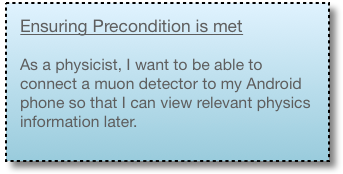
\includegraphics[width=0.7\textwidth]{storycard1.png}
  
\end{figure}

\begin{figure}[h]
  \centering
  
      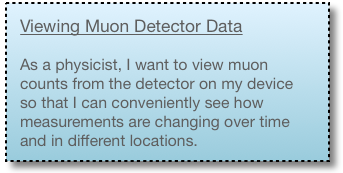
\includegraphics[width=0.7\textwidth]{storycard2.png}
     
  
\end{figure}

\begin{figure}[h]
  \centering
  
      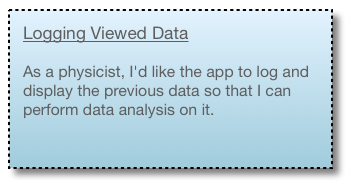
\includegraphics[width=0.7\textwidth]{storycard3.png}
      \caption{Individual story cards are first created to document core requirements, upon which further cards will be used to document how a user goes about accomplishing those tasks}
  
\end{figure}


\subsection*{2-3: Story Map}

With the use of the user story cards above, a collage/story map can be created that details further on how a user can interact with the app to accomplish their requirements. The story map can be viewed on the next landscape page;

\newpage
\begin{landscape}
\begin{figure}[h]
  \centering
  \vspace*{-2cm} \hspace*{-0.5cm}
      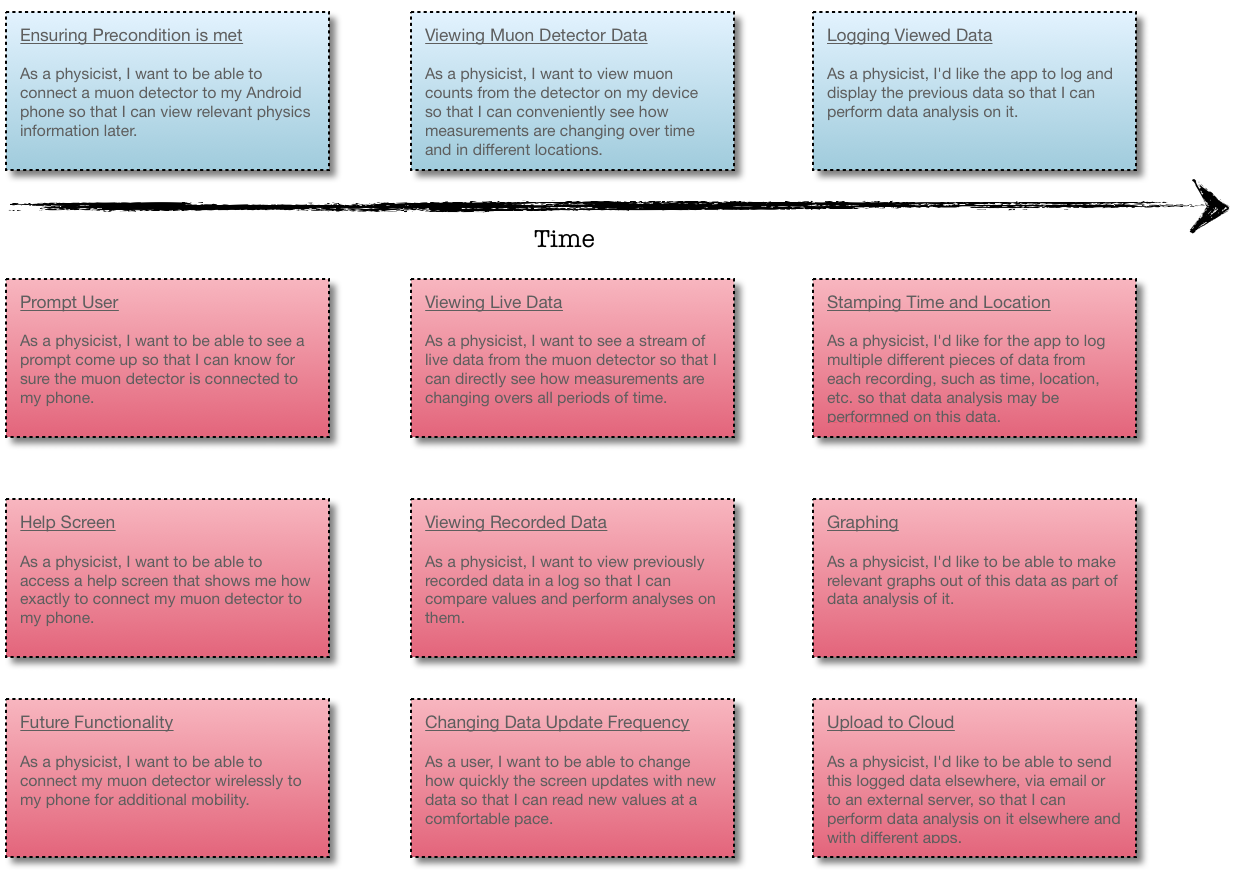
\includegraphics[width=1.9\textwidth]{storymap.png}
      \caption{A story map is used to organize requirements in order of priority and to illustrate how user interacts with app}
  
\end{figure}
\end{landscape}

\section*{Deliverable \#3}

\subsection*{3-1: Overview Sketches}
\bigskip
\begin{figure}[h]
  \centering
      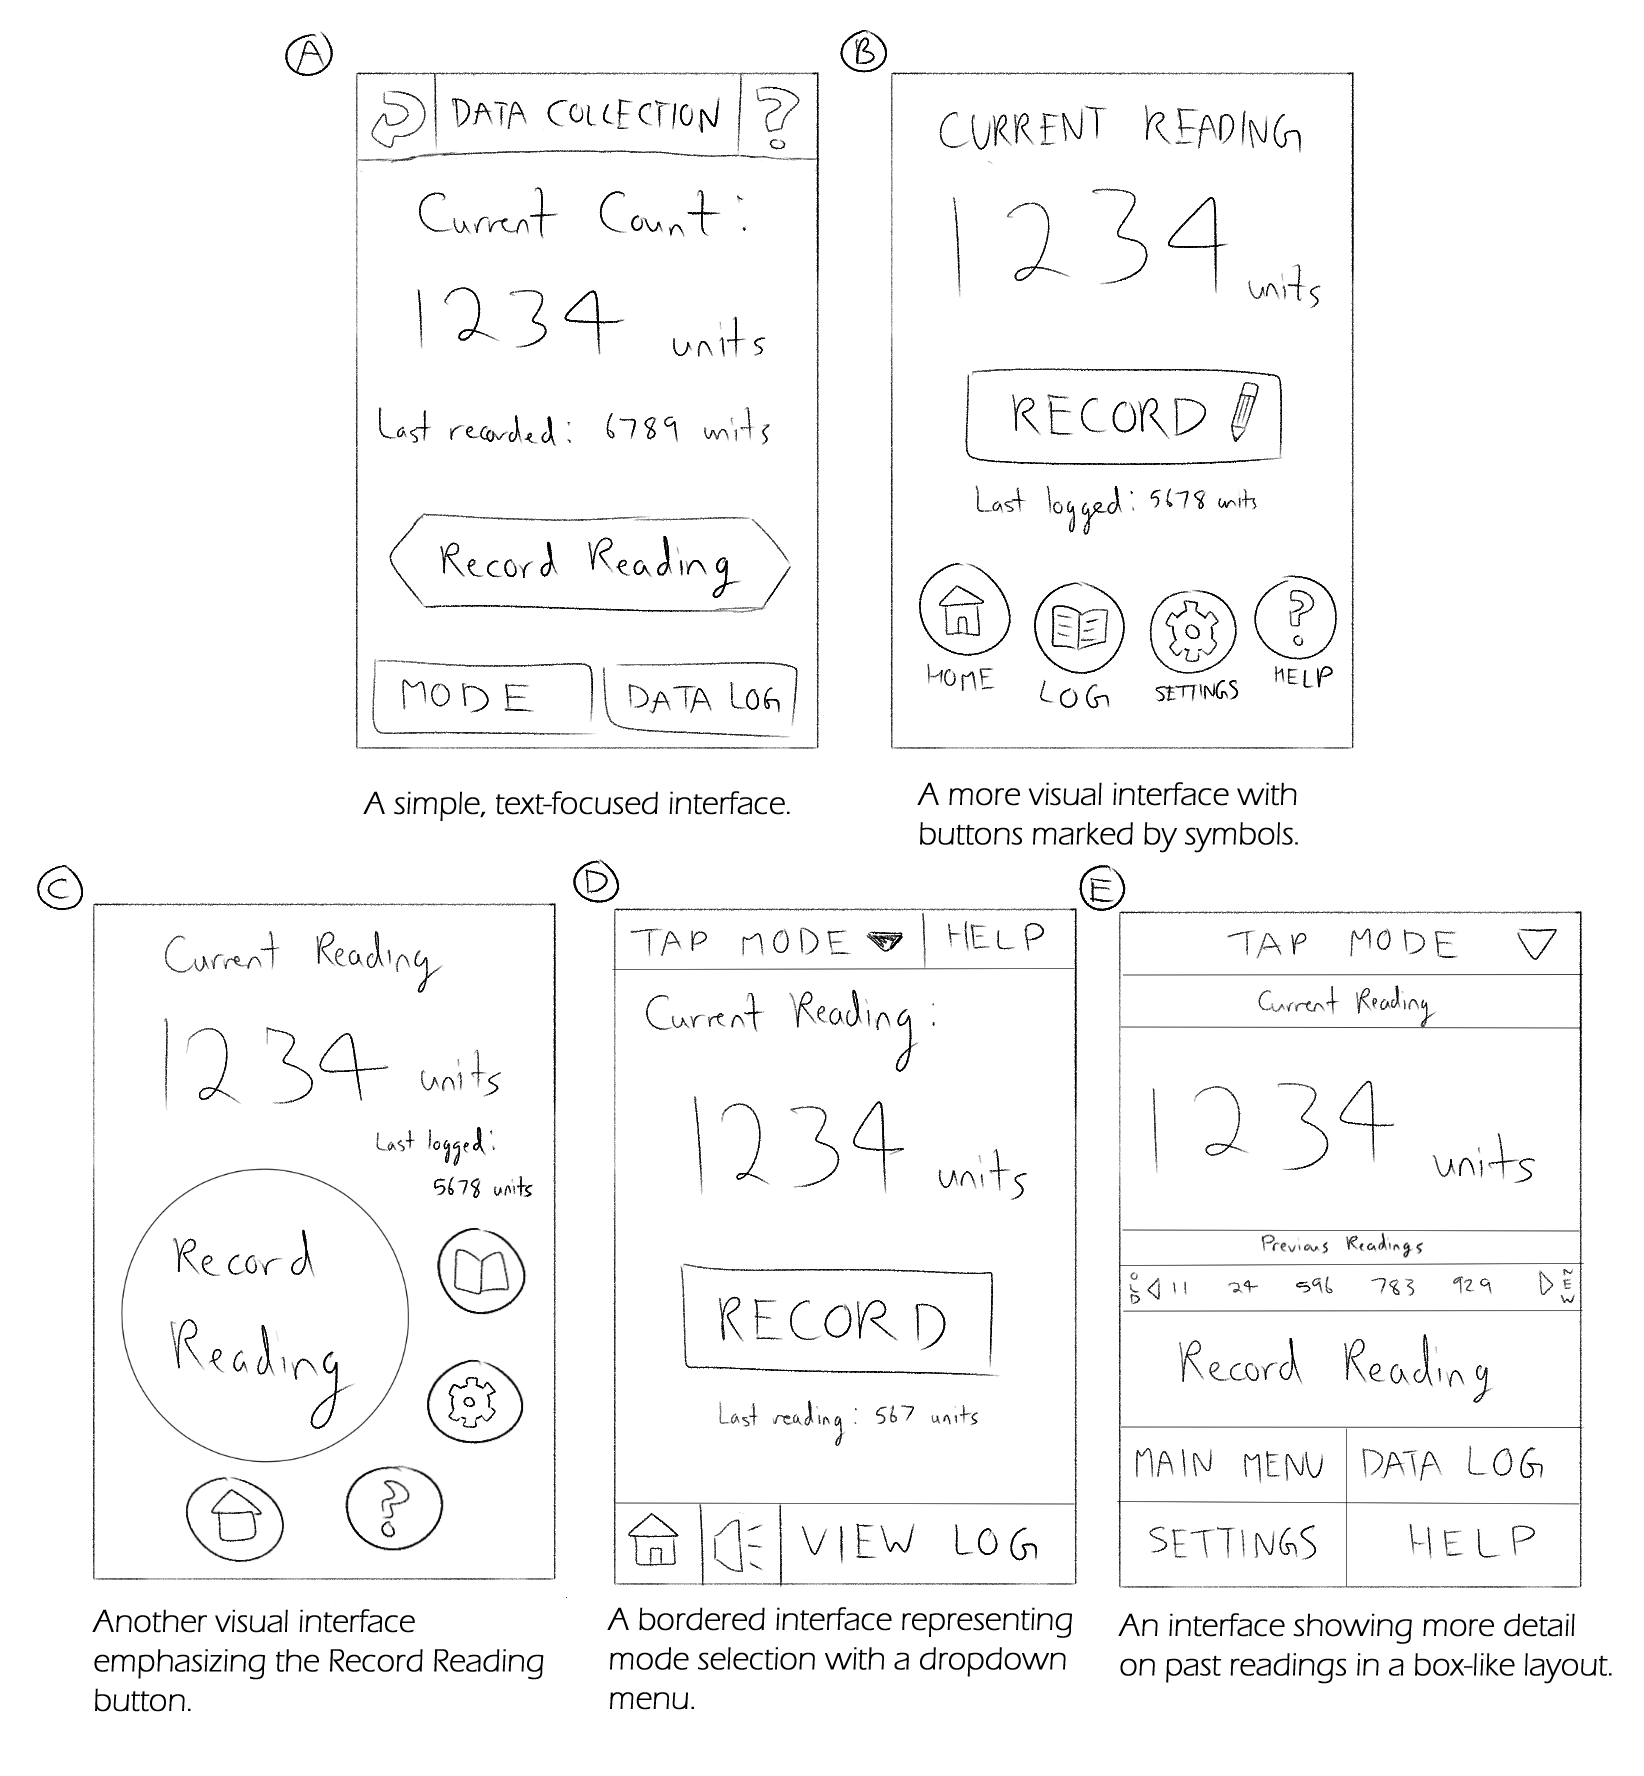
\includegraphics[width=1.1\textwidth]{overviewsketches.png}
  \caption{A variety of design approaches for the recording screen}
\end{figure}

\newpage
\subsubsection*{Why We Chose Sketch A}

We chose sketch A to elaborate on due to its clarity and emphasis on the most important aspects of this screen. The main buttons the user would interact with (Record, Mode and Data Log) are large and displayed clearly. Compared to sketches B and C, which have smaller icons that the user may accidentally mis-press, the interface of A is more focused on what is important to the user. This is key to enhancing the intuitiveness of the app. Sketch D emphasizes similar points to sketch A, but the mode selection button is somewhat less obvious in this design. Although sketch E shows more information about Previous Readings than the other sketches, it is too cluttered; additionally, that information is repeated in the Data Log screen in more detail, so it is not needed for the Data Collection screen. Thus, our main reason for choosing sketch A was its relative simplicity and correctly emphasized functions compared to the other designs.

\subsection*{3-2: Elaborating Sketches}
\def\textfraction{.01}
\def\topfraction{.99}
\bigskip
\begin{figure}[b!]
  \centering
  \hspace*{-1cm}
  \renewcommand{\textfraction}{0.05} 
      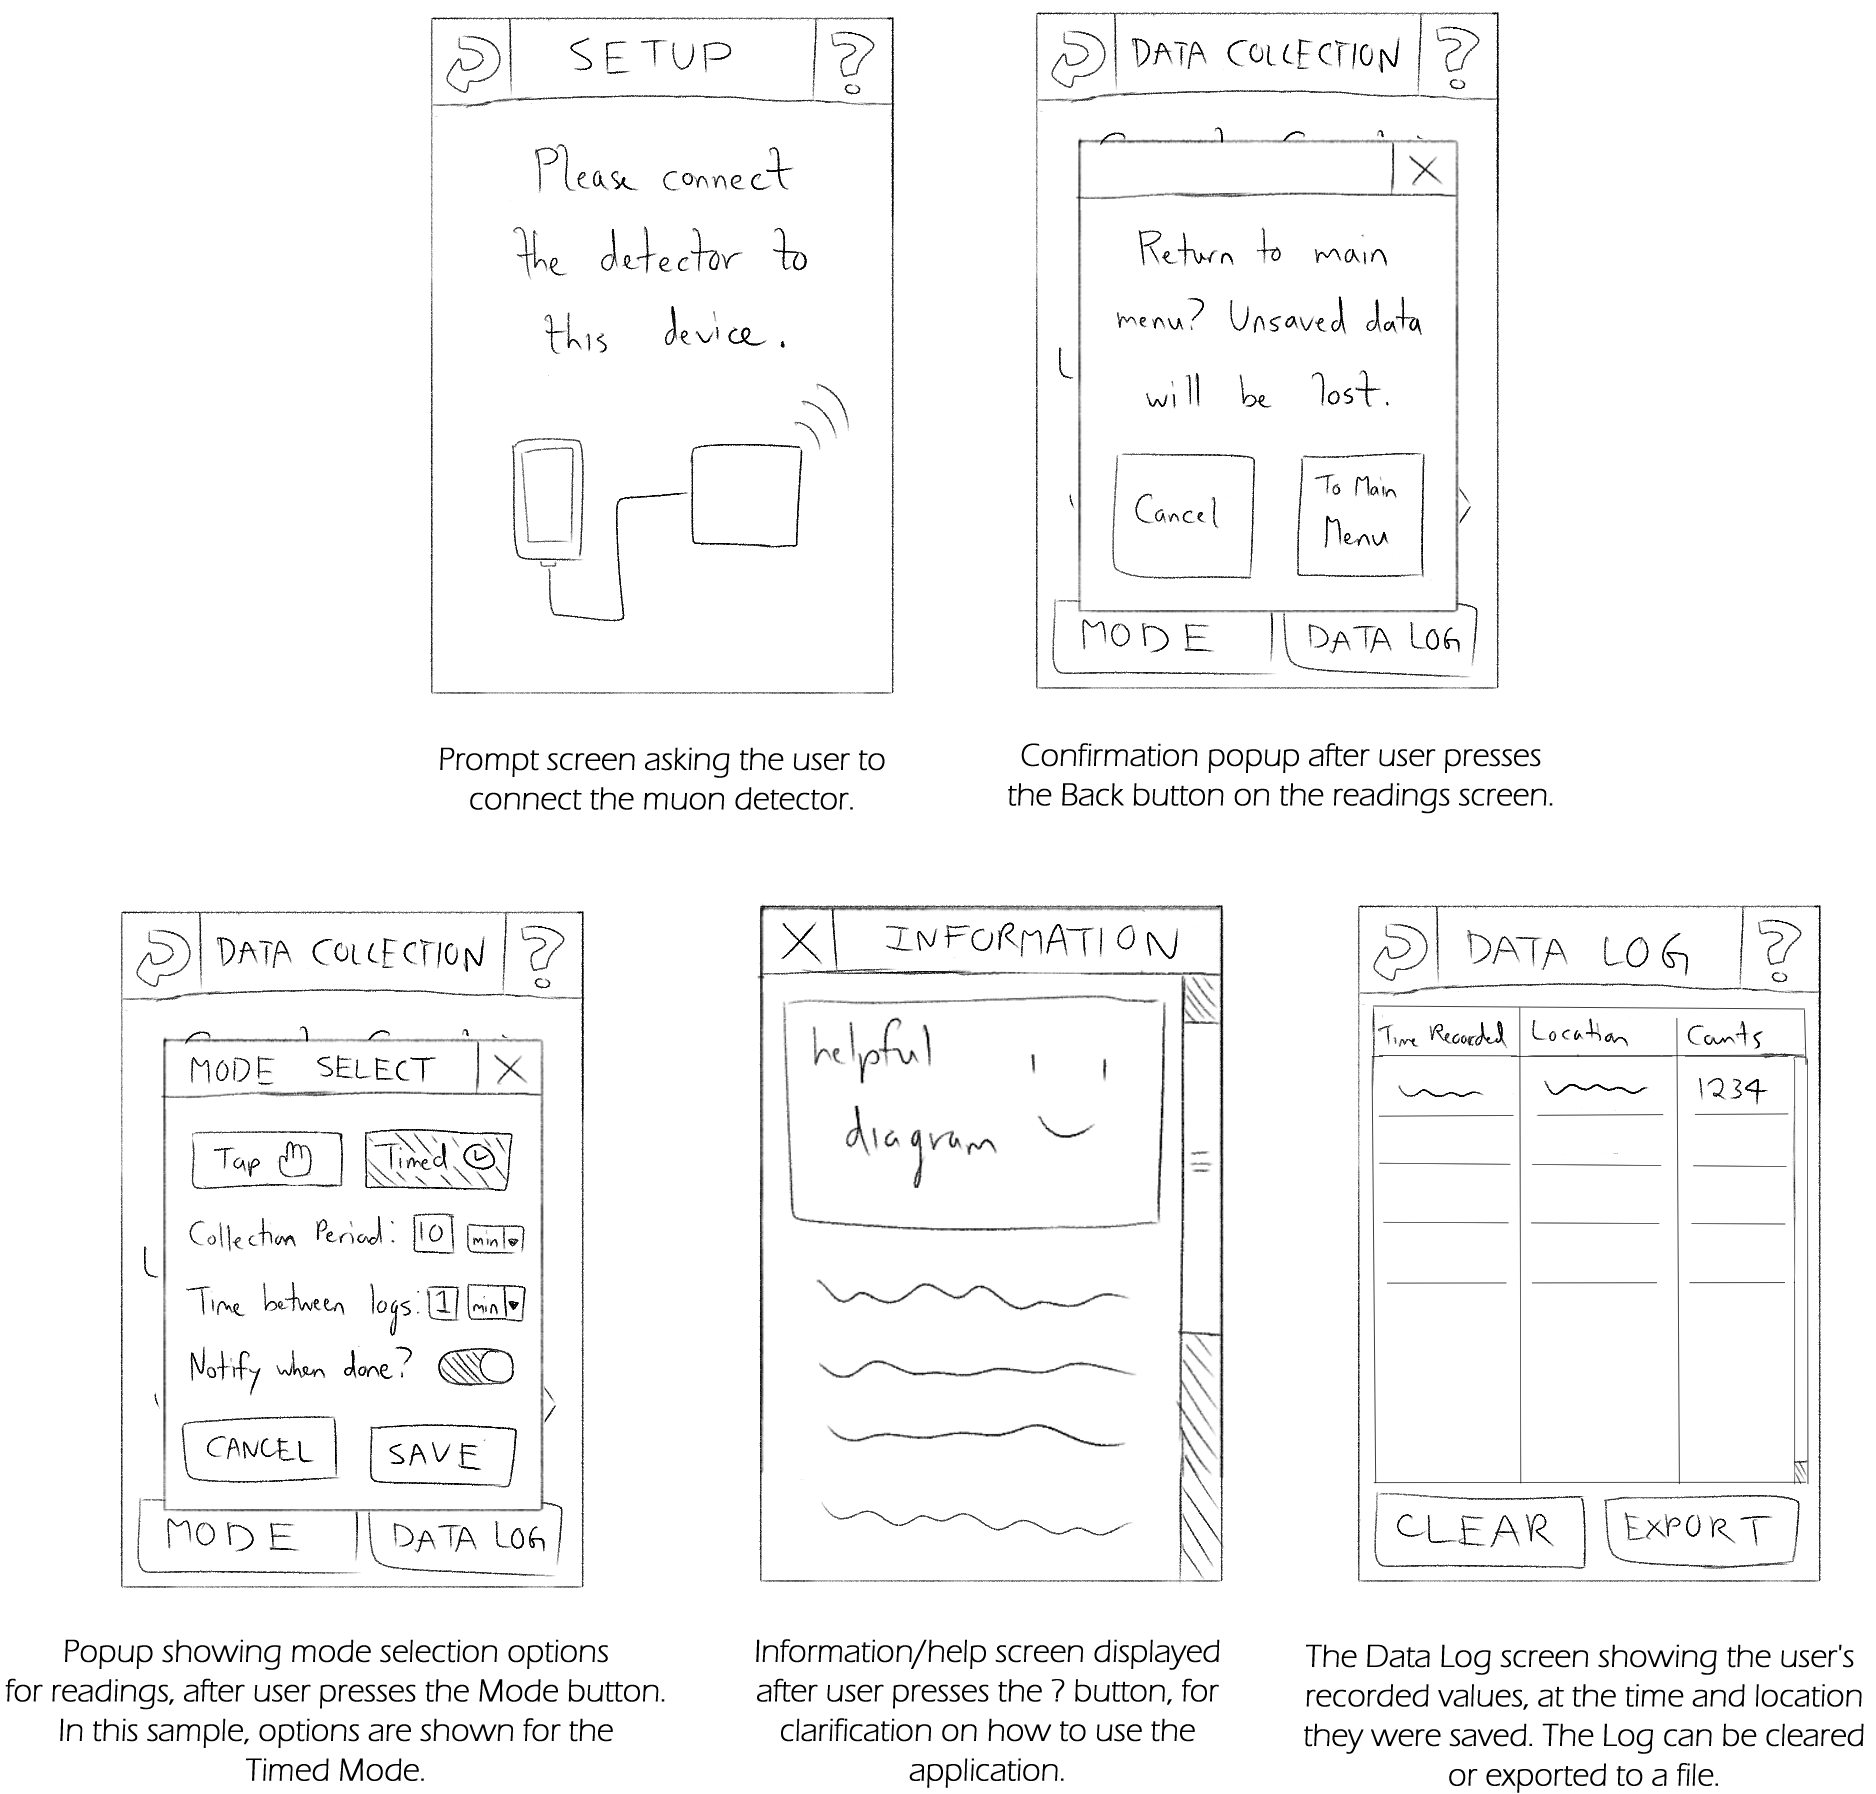
\includegraphics[width=0.84\textwidth]{elaboratingsketches.png}
  \caption{Extended sketches for other parts of the apps UI screens}
\end{figure}

\newpage
\subsection*{3-3: Storyboard Sketches}

\bigskip
\begin{figure}[h]
  \centering
  \hspace*{-0.5cm}
      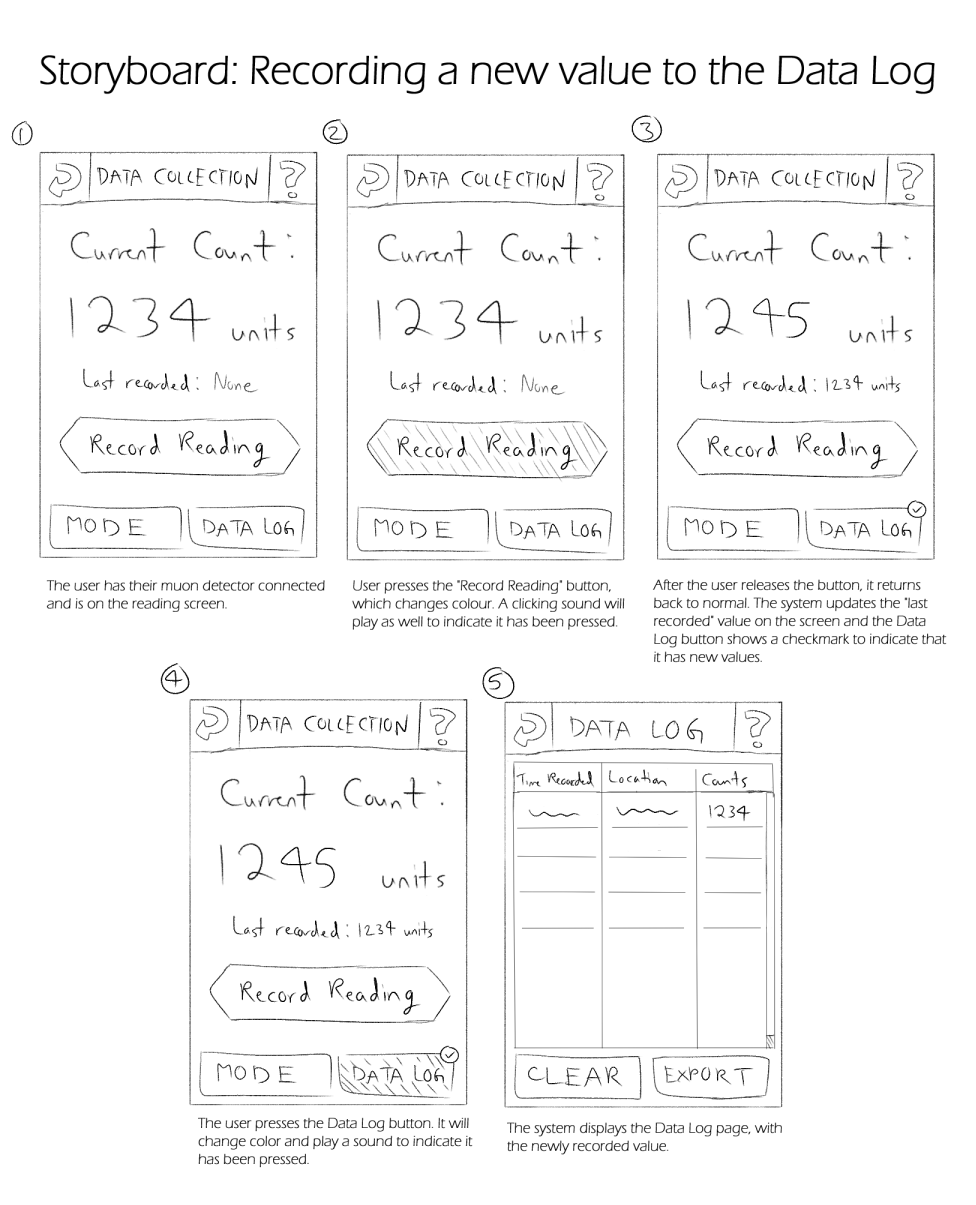
\includegraphics[width=1.15\textwidth]{storyboard.png}
  \caption{The recording screen responding to user input}
\end{figure}

\newpage
\subsection*{3-4: Wizard of Oz Demo Video}

Demo videos can be viewed below:

1. Full Video 30min (\href{https://drive.google.com/file/d/1D5OwAUCmAK5fYUDqaYs4WdFURqq9lxwS/view}{\underline{link}})

2. Short Video 1min (\href{https://drive.google.com/file/d/1GZPQ2MqETNLw6sNSMTrlxhX4ftYG58Hb/view?usp=sharing}{\underline{link}})






\section*{Deliverable \#4}
\subsection*{4-1: Poker Effort Estimation}

For our planning poker session, we chose to create tasks for the following functional requirement:

\textbf{The app must process event data from the muon detector to determine the number of events per minute over a specific time interval.}

We generated six tasks for this functional requirement and individually rated the difficulty of each task from one to ten. During our planning session, we generally had consensus for our ratings, with some variance between us. 

For example, the task, “Create an addEvent method to store processed MuonEvents to an array”, was considered to be relatively easy by all of us. However, one person rated the difficulty slightly higher and suggested that this method may need to check if the event data is valid (eg. if the timestamps are in an order that makes sense). We discussed some other issues that may occur, such as what should happen if a maximum number of events had been reached. These additional factors helped clarify the difficulty of the task.

The task of “calculating the difference in minutes between two timestamps” was more divisive. One of our group members believed the task would be quite difficult (7) but another believed it would be easy (3), since Java likely contained some built-in functionality to help with the task. We learned that this was indeed the case and adjusted our rankings accordingly.
We all agreed that the task of “calculating events per minute over a specific time interval” would be difficult. During our discussion, we contemplated how the number of events per minute could be displayed “live” on our app screen while collecting data, since that would involve frequently saving new timestamps for the calculation. We also wondered if events per minute should only be calculated over some fixed time interval (eg. the last 10 seconds of recording) or use the whole time spent recording.

Overall, the planning poker session was useful for evaluating our list of tasks by raising new questions on generating ideas for test cases and structure.


\subsection*{4-2: Silent Grouping Effort Estimation}

Once our planning poker session was completed, we moved along to do silent grouping effort estimation. We now had to define features of the functional requirement rather than the tasks. The definition of a feature we used was an element the user can see or interact with, corresponding to the functional requirement defined in \textit{Deliverable 1-1}. The features we came up with were:

\begin{enumerate}

\item The user is able to press the 'Start Recording' button to begin when data collection starts.
\item The user is able to see events being displayed on the recording screen after each new event is detected and added.
\item The user is able to stop the recording midway if desired.
\item The user is able to clear the screen once a session is done to start a new recording session.
\item The user is able to see when a recording is in progress by noticing the green Start Recording button changes into a red Recording (duration remaining in s) button.
\end{enumerate}

After coming up with the above list, we wrote them down on some post-it notes and used a table rather than a wall to do the sorting;

\begin{figure}[h]
\centering
	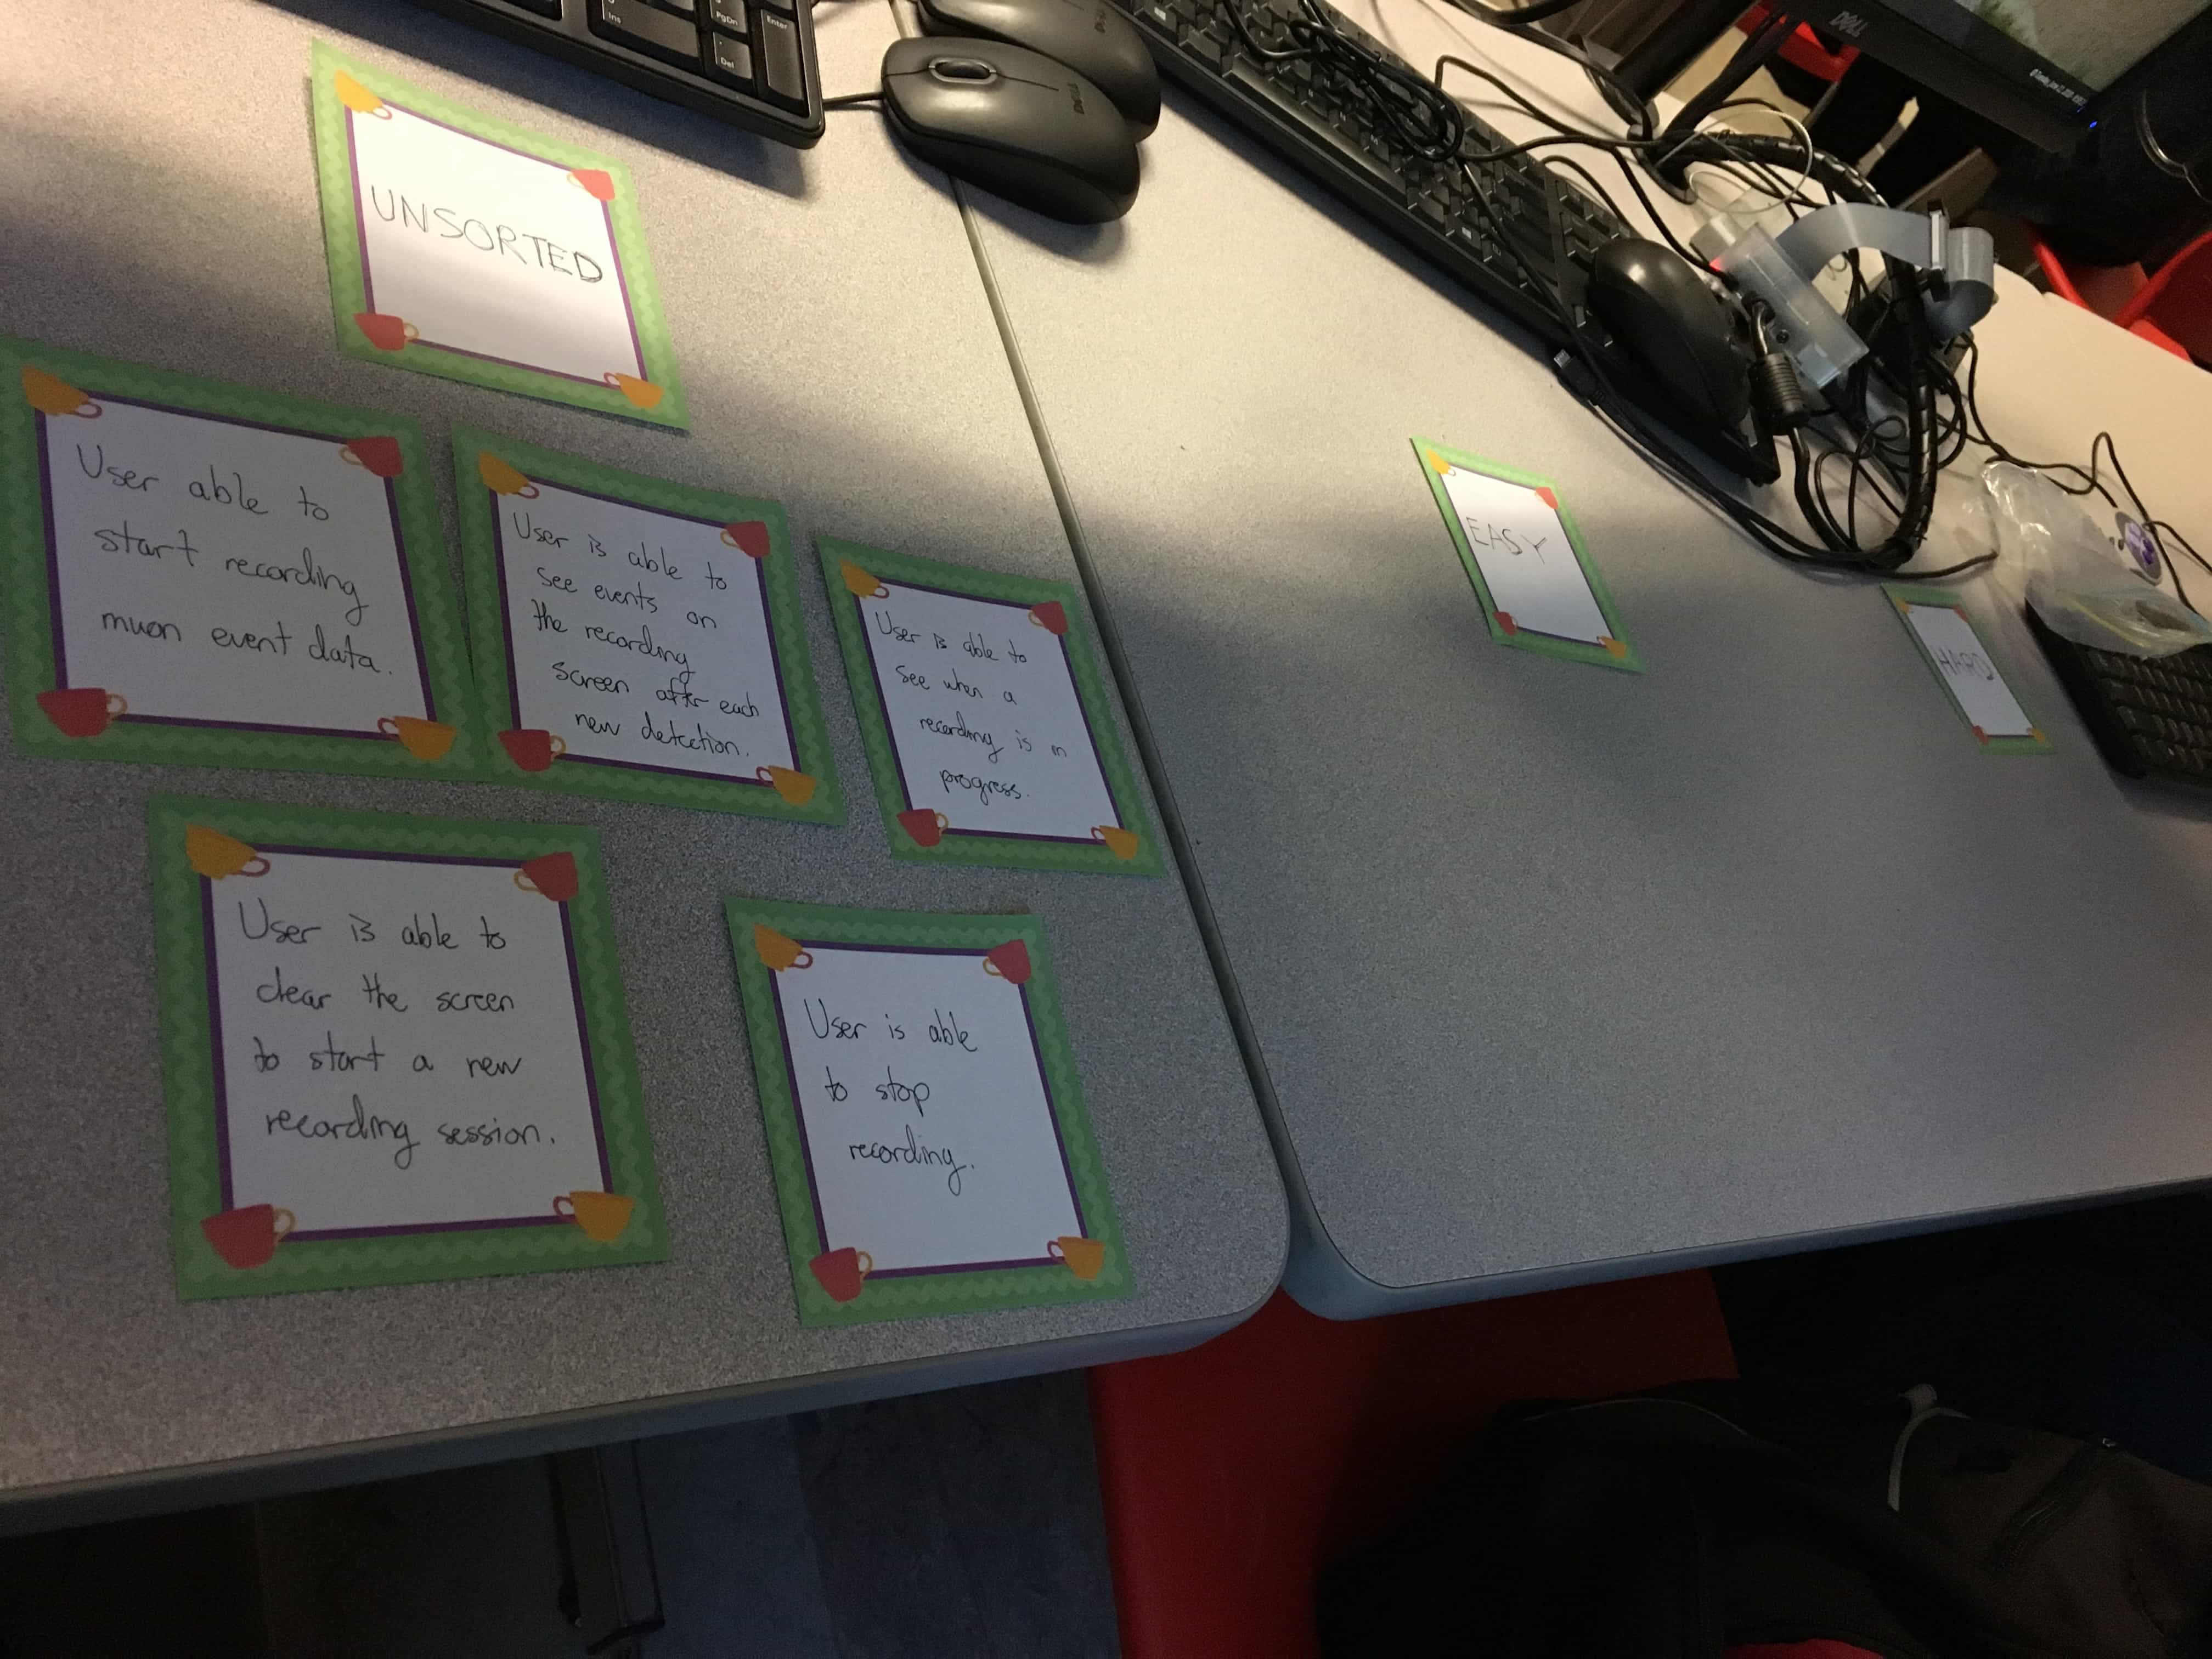
\includegraphics[width=0.9\textwidth]{silentimg1.png}
	\caption{Post it notes started initially in the unsorted pile and a table was used for convenience}
\end{figure}

\newpage

One of the issues we noticed with the silent grouping method was the lack of granularity of the piles. A feature was either easy or hard whereas the planning poker method was able to give a finer sense of difficulty. As such, clearly easy or hard features were the first to get picked and sorted which is seen in the below in progress shot; 

\begin{figure}[h]
	\centering
	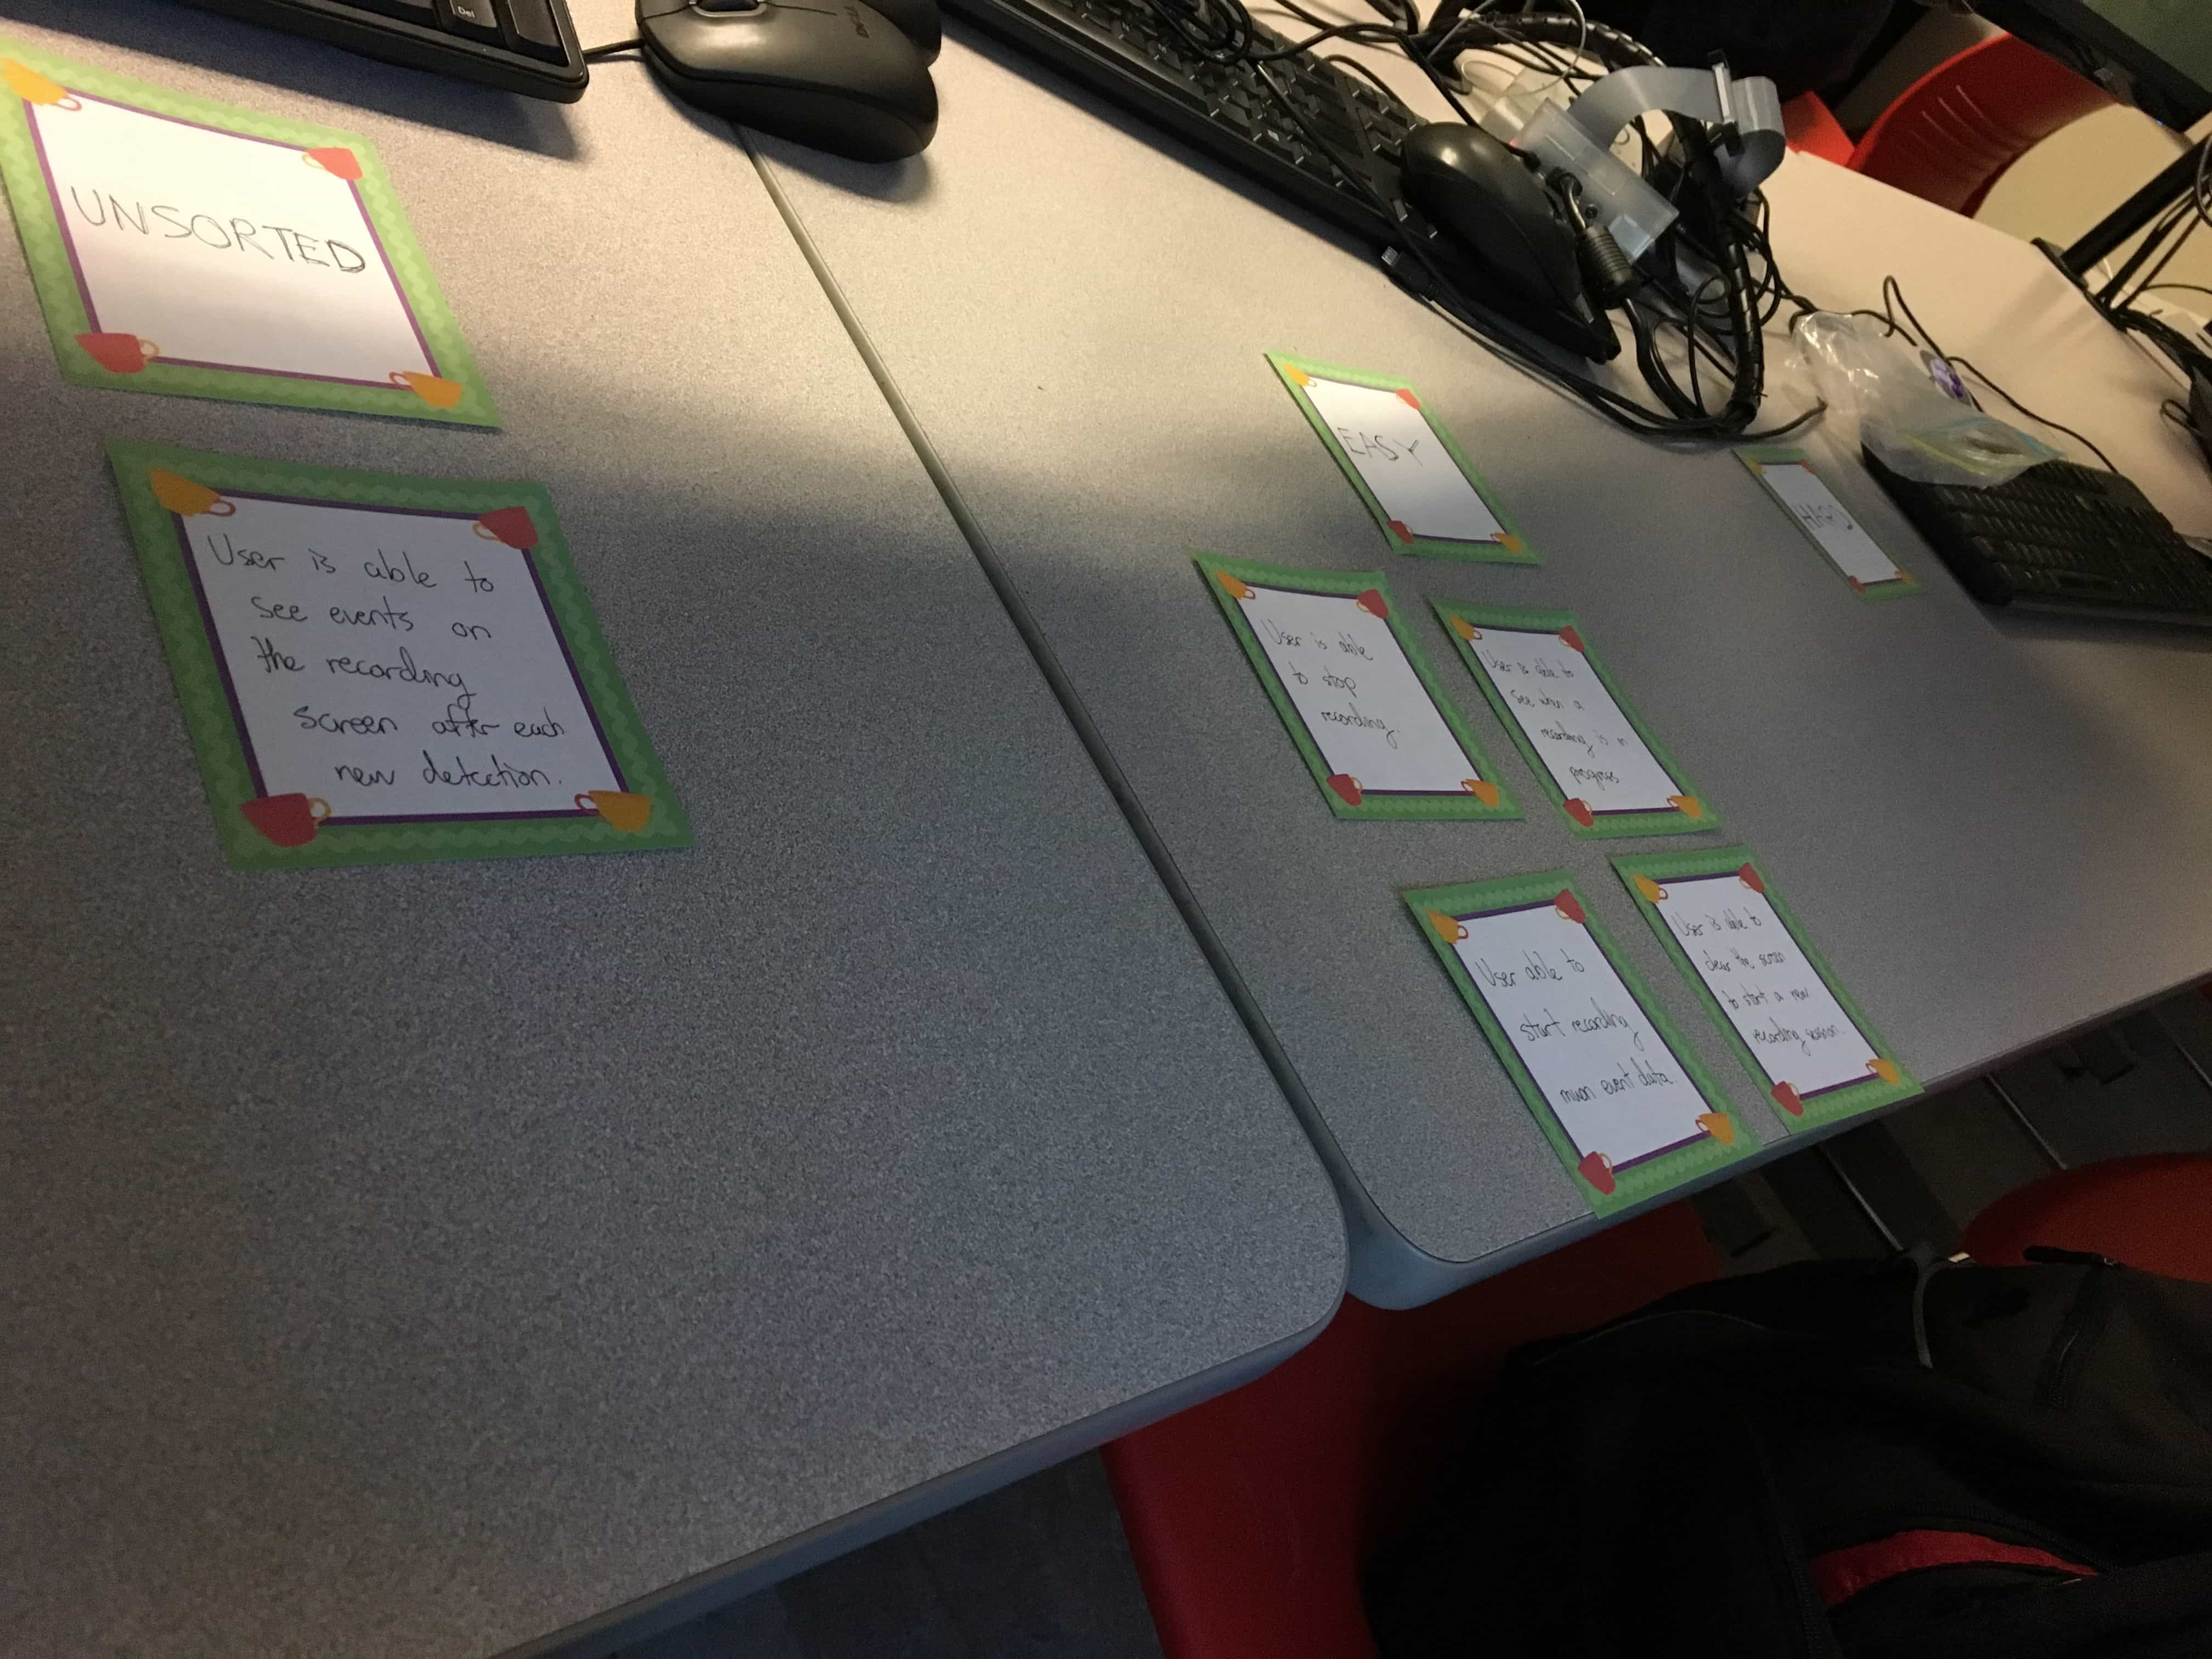
\includegraphics[width=0.5\textwidth]{silentimg2.png}
	\caption{Silent grouping effort estimation in progress}
	\end{figure}

We then attempted to categorize some of the harder features such as displaying the live event being detected and added to a running total. This aligned with our previously defined hard task in \textit{Deliverable 1-1} and a consensus was reached that this would indeed be difficult. 

Afterwards, a feature that was hard to reach an agreement on was stopping the recording half way. Stopping it mid way may prove to be difficult so after a few back and forth for that feature, we decided to put it in a middle 'hold' section as seen below:

\begin{figure}[h]
	\centering
	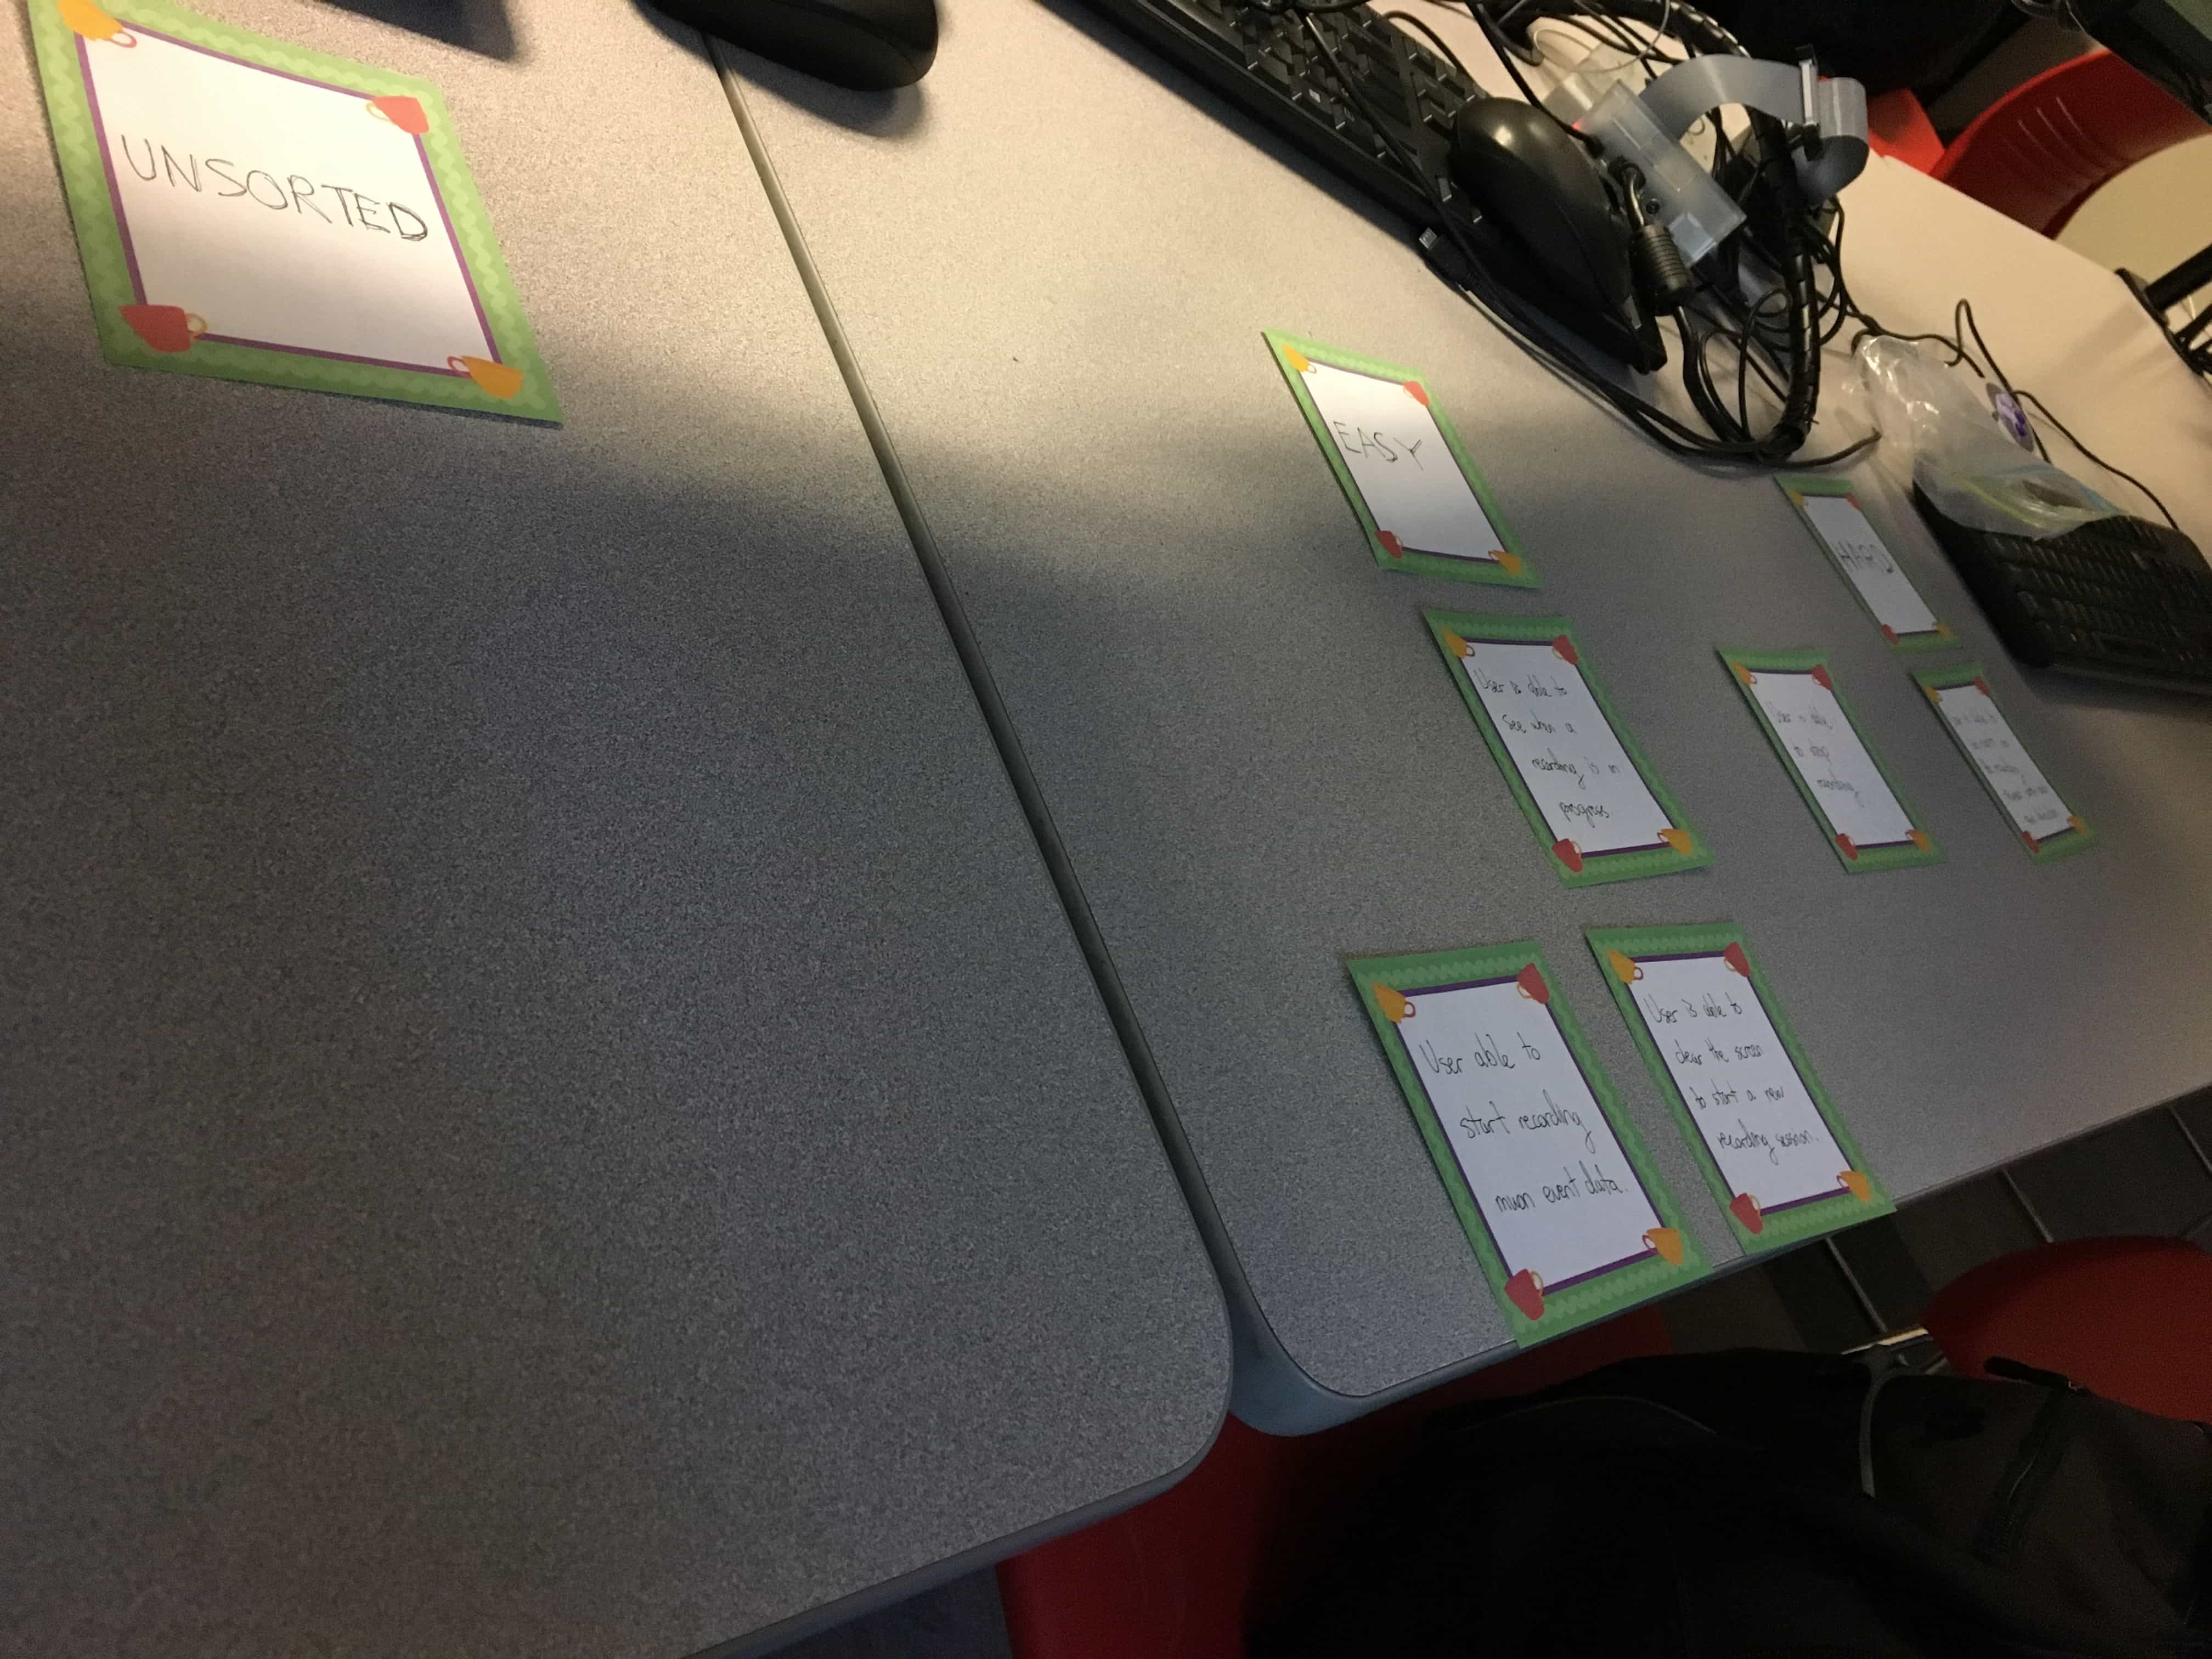
\includegraphics[width=0.5\textwidth]{silentimg3.png}
	\caption{Completed session with one of the features being placed on hold}
	\end{figure}
	
Overall, silent grouping  proved to be a valuable medium of communication in allowing team members to interact with one another. An exchange of different views can ultimately help in creating a better application. 


\newpage
\subsection*{4-3: Task Breakdown}

\begin{figure}[h]
  \centering
      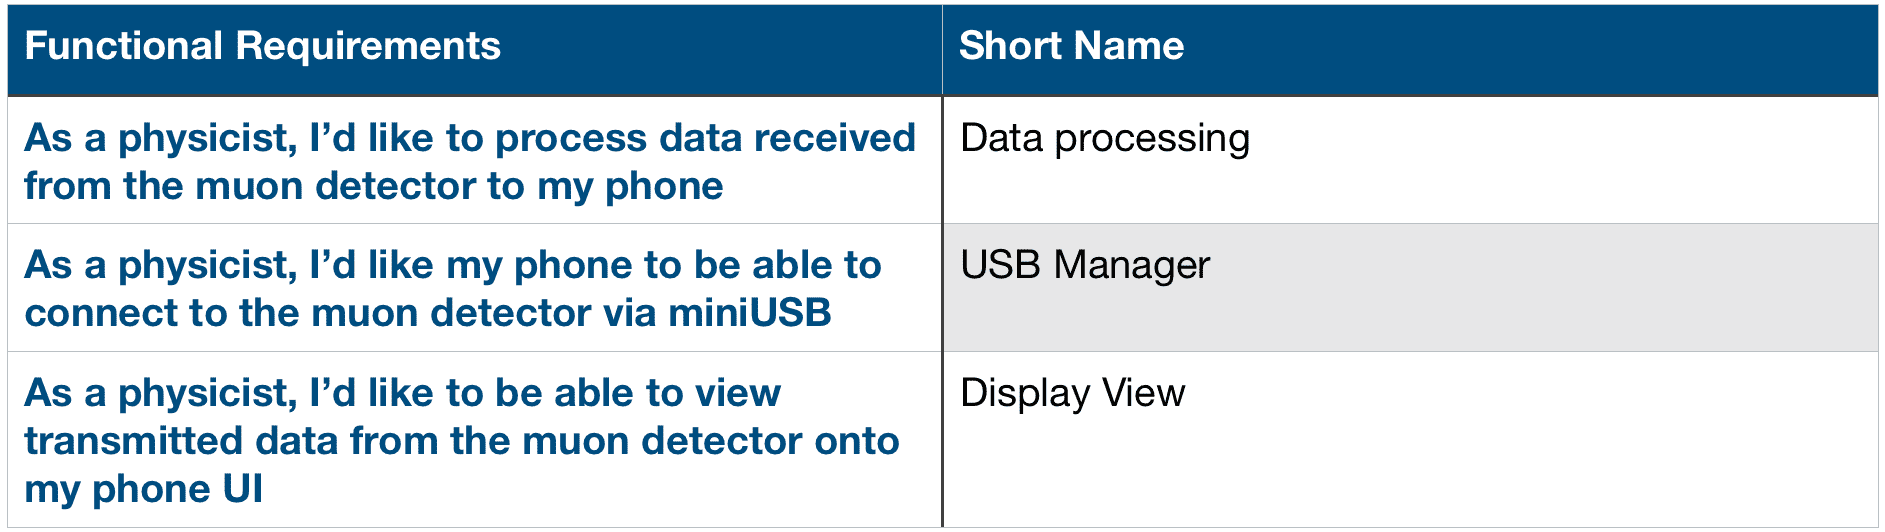
\includegraphics[width=1\textwidth]{table1.png}  
\end{figure}

Our first table shows the three main functional requirements picked for the app and their corresponding short names to be used in the following tables.

\begin{figure}[h]
  \centering
      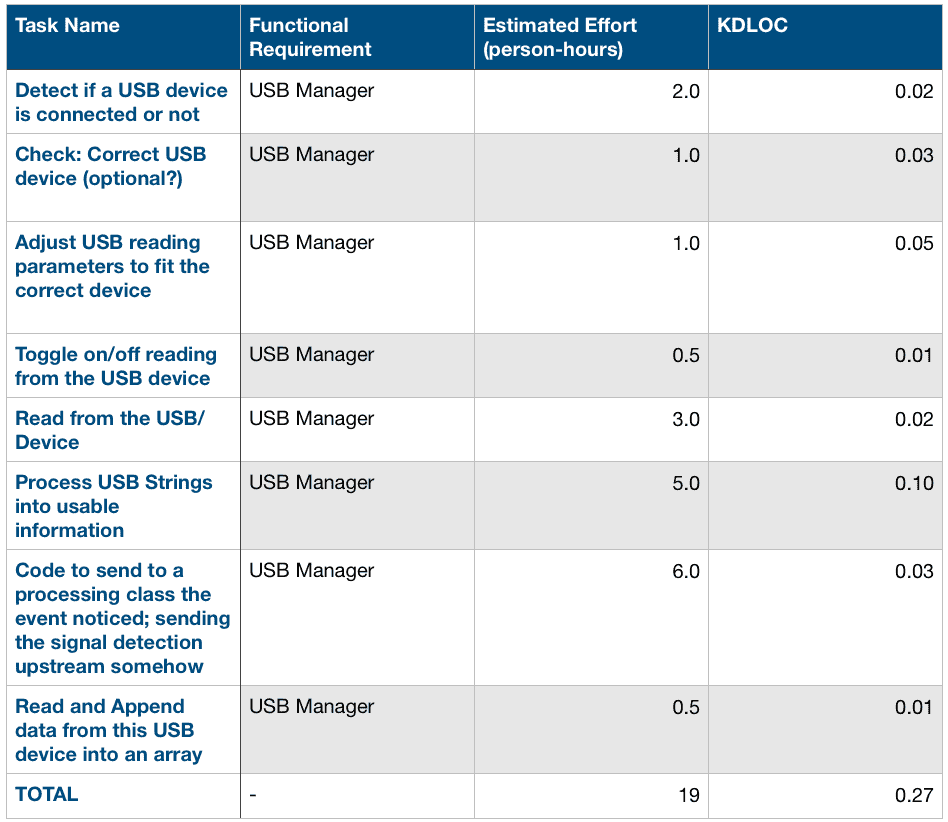
\includegraphics[width=1.0\textwidth]{USBMtable3.png}  
\end{figure}

Our second table corresponds to the USB Manager functional requirement. The table format serves as a visual aid for breaking down requirements into tasks and effort, which also provides a documentation reference in the future for cost estimation. 

\newpage
\begin{figure}[h]
  \centering
      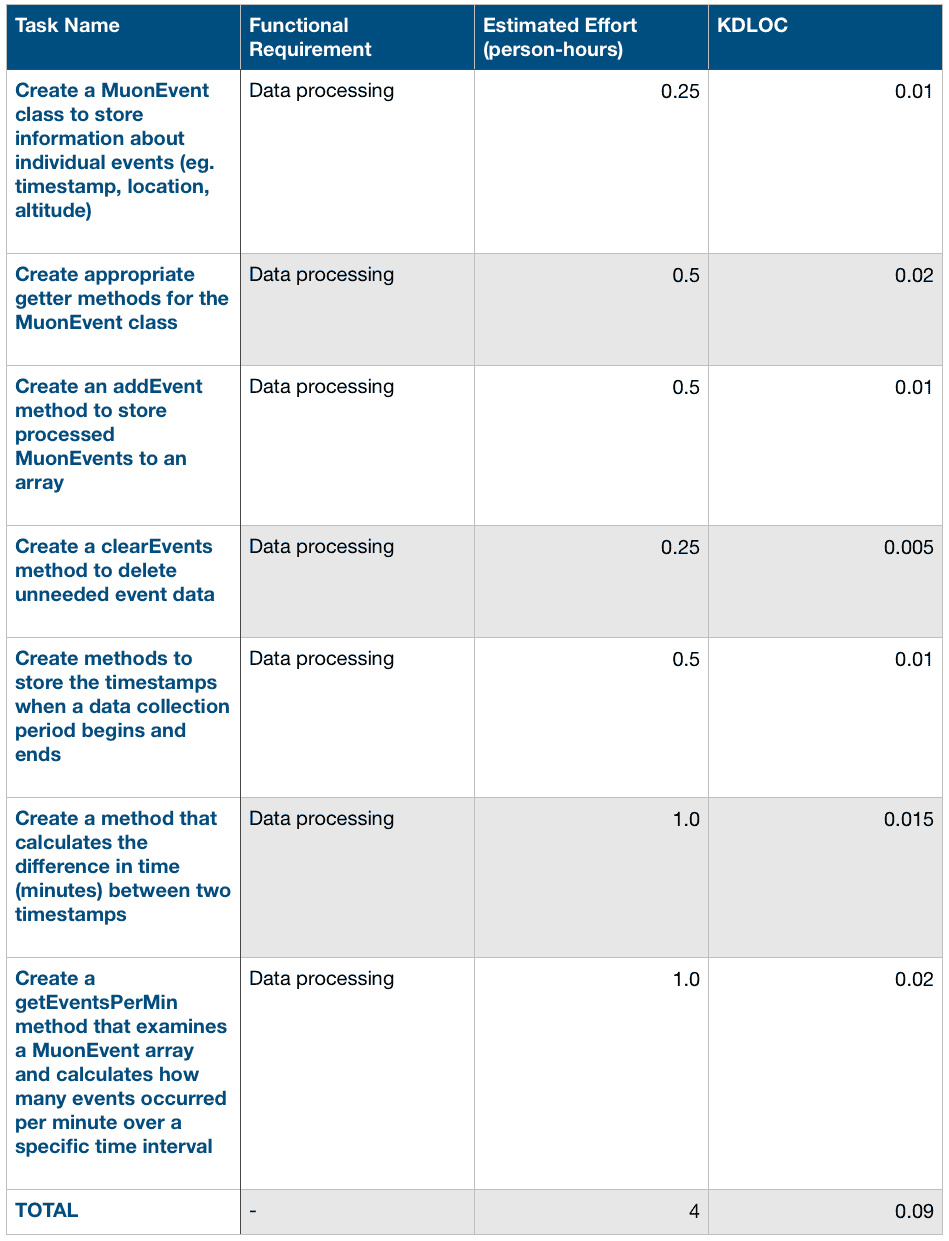
\includegraphics[width=1.0\textwidth]{dataproctable2.png}  
\end{figure}

Our second requirement is similarly broken down into individual tasks and their corresponding estimated effort.

\newpage
\begin{figure}[h]
  \centering
      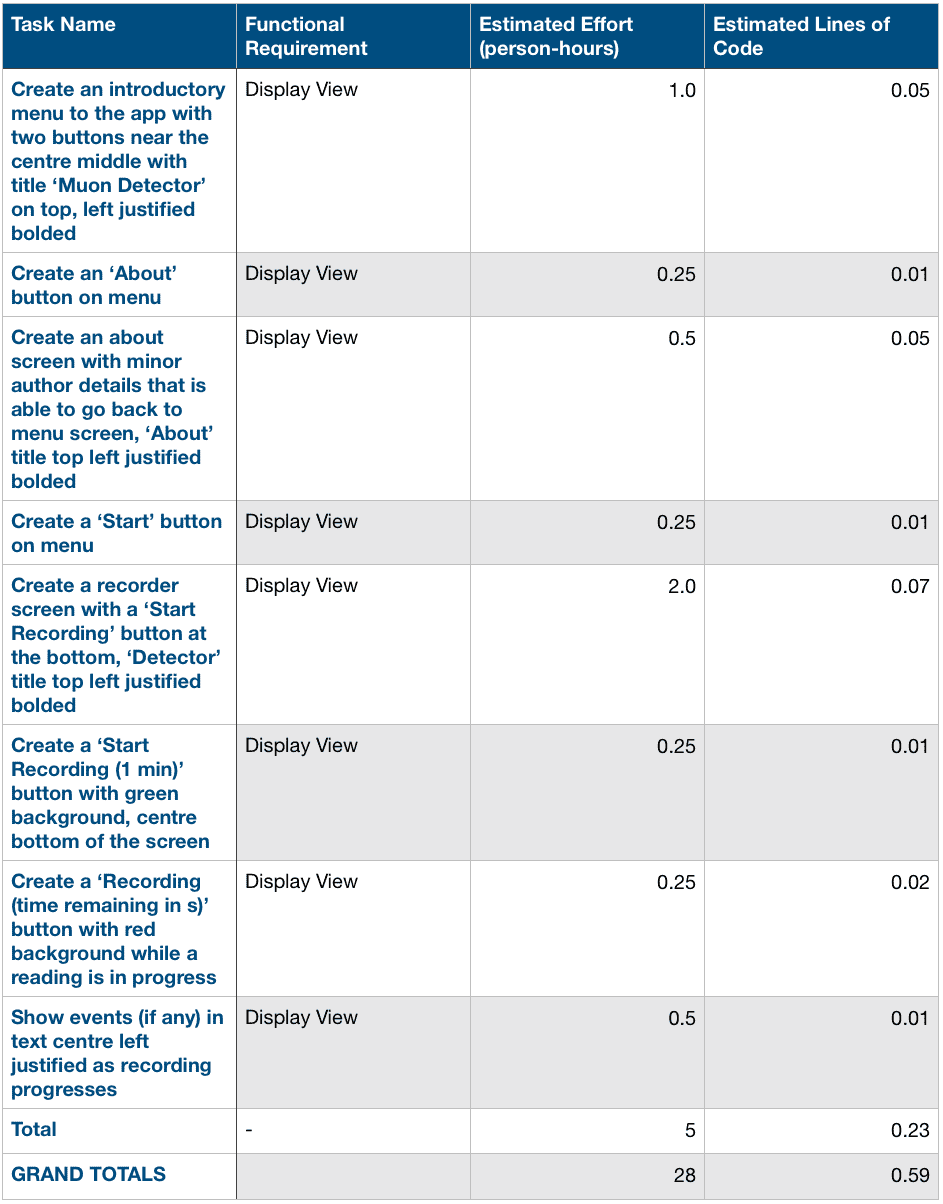
\includegraphics[width=1.0\textwidth]{displaytable4.png}  
\end{figure}

Finally, our third table for the final display functional requirement is also broken down. 

Overall, this exercise in the design process helped create estimates on the challenges to be faced when completing functionality of the application. This also helped plan our schedules since we now had a general idea of time required for each step. 



\newpage
\section*{Deliverable \#5}

\subsection*{5-1: Initial Tests}

For the data processing requirement, we will focus on testing the Processor class. This class will store event data as MuonEvents occurring over some time period. Here, we see seven initial test cases that focus on checking if the correct number of events have been stored (by the getEventCount() method) and on calculating the number of events per minute. None of the test code is complete save for the expected values:

\begin{figure}[h]
      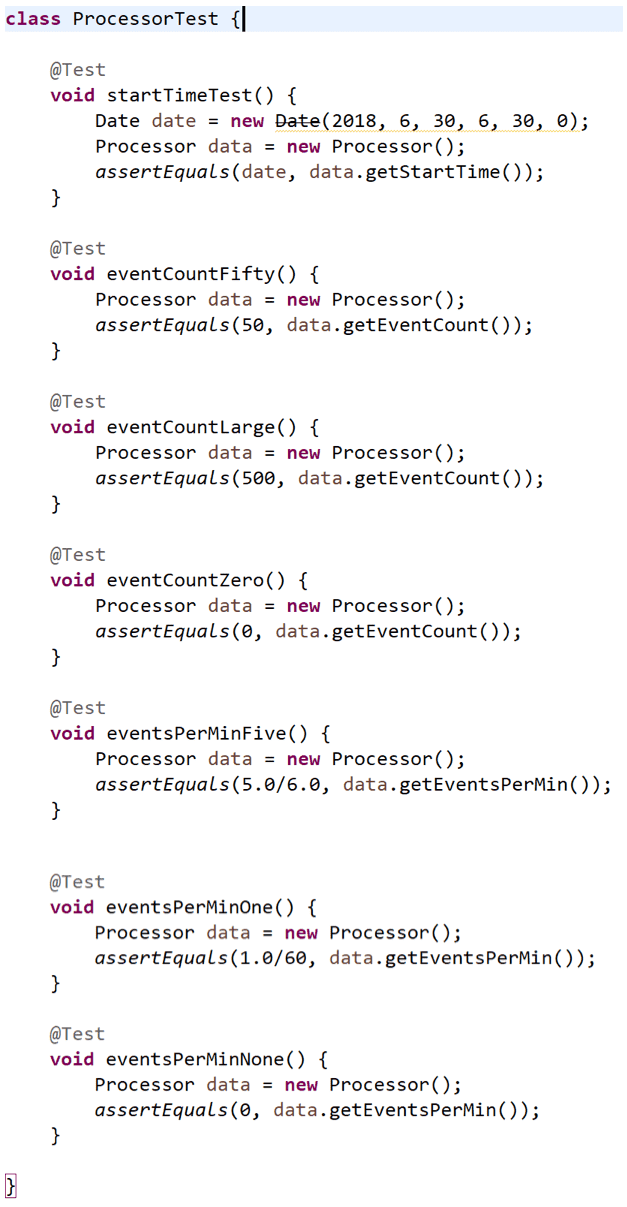
\includegraphics[width=0.63\textwidth]{codeimg1.png}  
\end{figure}

To compile the test code, a basic skeleton of the Processor class was created:

\begin{figure}[h]
	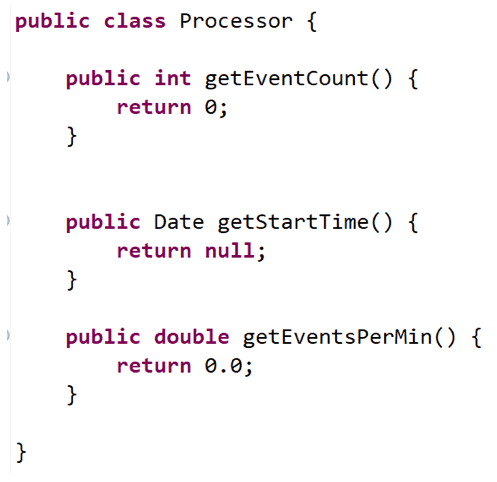
\includegraphics[width=0.63\textwidth]{codeimg2.png}
\end{figure}

When the previously created test class was now run, all but two of the tests failed. The only tests that passed already expected "0" as a result:

\begin{figure}[h]
	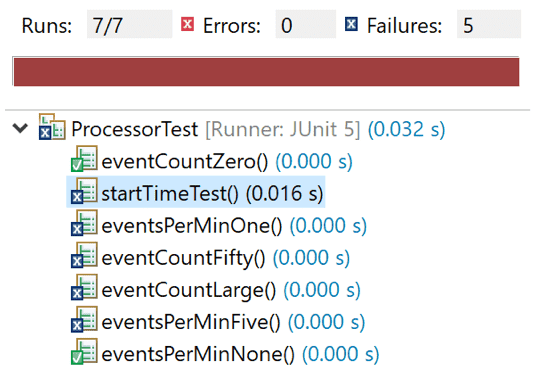
\includegraphics[width=0.83\textwidth]{codeimg3.png}
	\end{figure}
	
\newpage
\subsection*{5-2: Tests with Partial Implementation}

While working on the implementation, we realized that we needed more data and methods to flesh out the Processor class, resulting in an increased number of test cases. For example, to calculate events per minute, we needed to save the timestamps when data collection began and ended to know the length of time spent recording data. This functionality is performed by the new switchRecording method.
 
Although the full implementation of this requirement will use real muon event data from a connected muon detector, the test cases created fake data to simulate how real events would be saved by the Processor.

The following screenshots show some of the test cases after implementation:



\begin{figure}[h]
	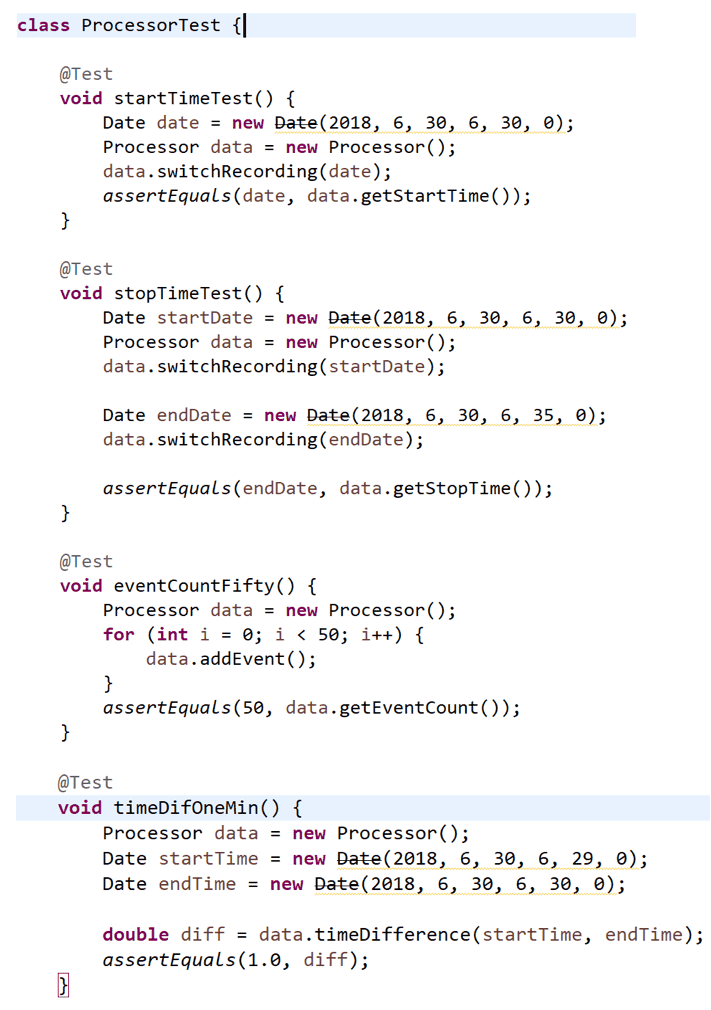
\includegraphics[width=0.79\textwidth]{codeimg4.png}
	\end{figure}

The new timeDifference method was created to calculate the difference between two timestamps in minutes. This is used in conjunction with the getEventsPerMin method:

\begin{figure}[h]
	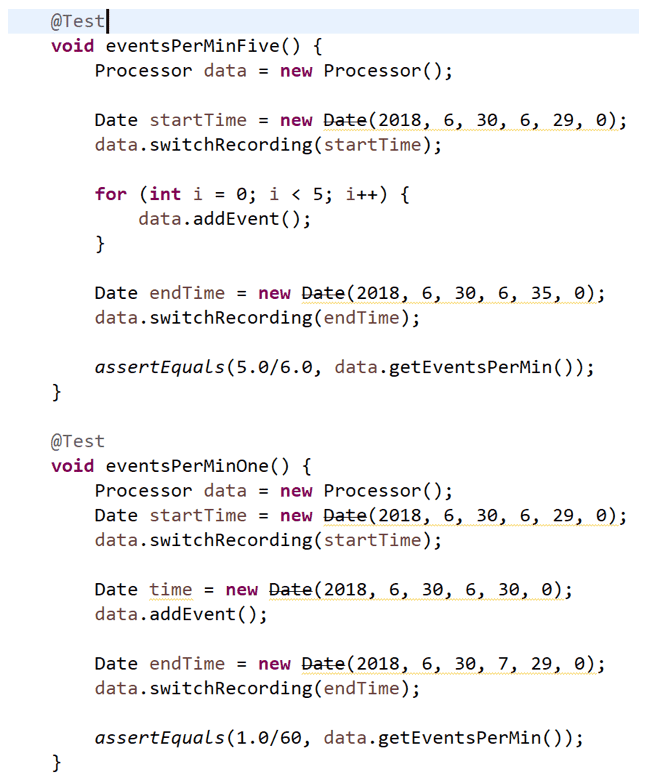
\includegraphics[width=1.0\textwidth]{codeimg5.png}
	\end{figure}
	
	
\newpage
The Processor class now has partially complete methods. However, it does not yet store instances of each muon event:

\begin{figure}[h]
	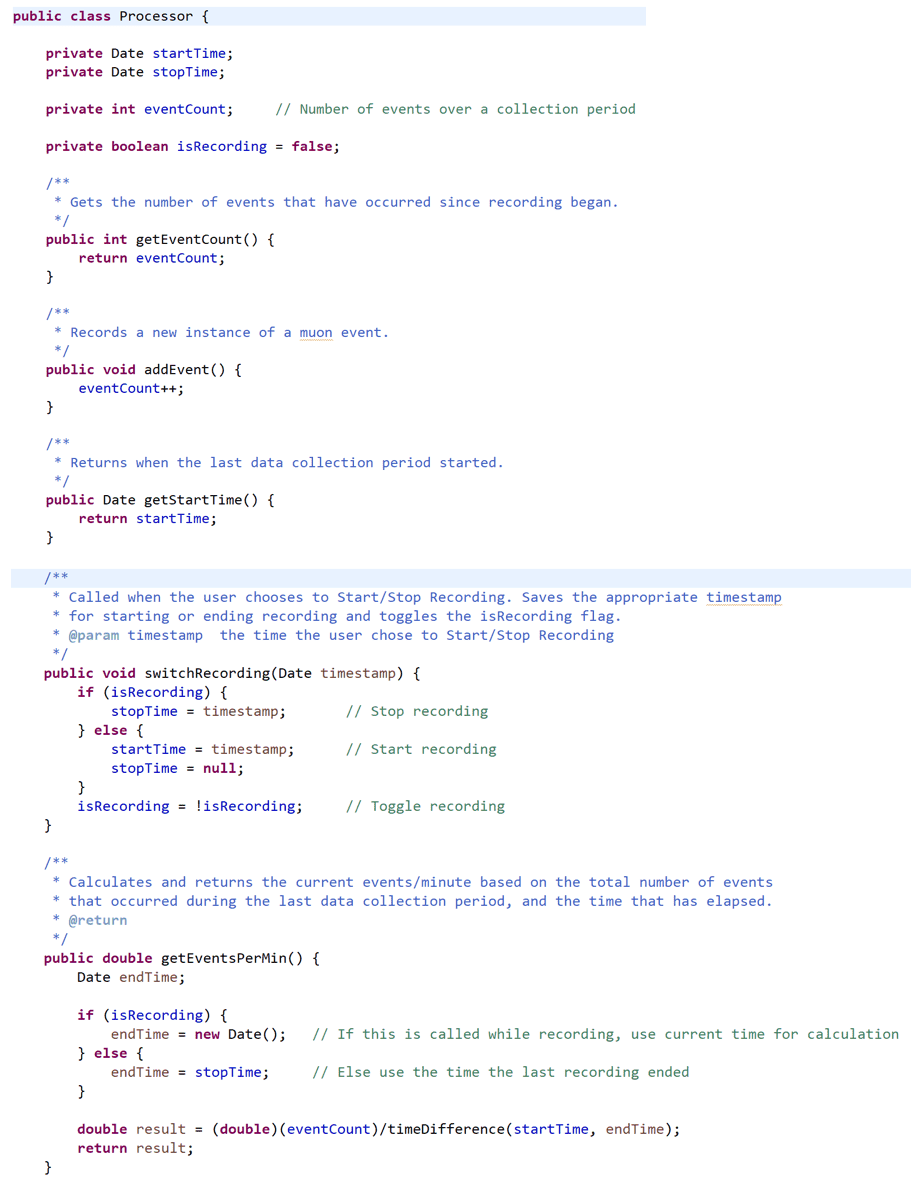
\includegraphics[width=1.1\textwidth]{codeimg6.png}
\end{figure}

\newpage

Now there is enough code to pass all the test cases:

\begin{figure}[h]
	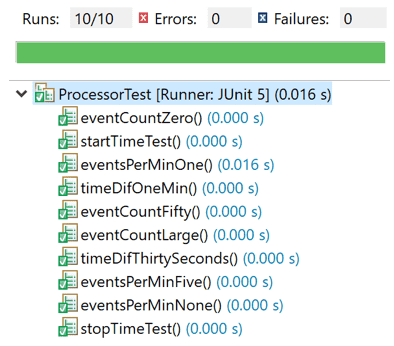
\includegraphics[width=0.7\textwidth]{codeimg7.png}
\end{figure}


\subsection*{5-3: Tests with Full Implementation}

Our demo video demonstrating the TDD approach with full implementation along with explanations can be viewed at the following (\href{https://www.youtube.com/watch?v=h2C-4-hQrhM&feature=youtu.be}{\underline{link}}).

\subsection*{5-4: Two Extra Functional Requirements}

Our demo video featuring all three functional requirements can be viewed at the following (\href{https://www.dropbox.com/s/vnuvuzx5zrtkvaa/Demo.mp4?dl=0}{\underline{link}}).



\newpage


\section*{Deliverable \#6}

\subsection*{6-1: Class Diagram}

\begin{figure}[h] \centering \hspace*{-3cm} \vspace{3cm}
	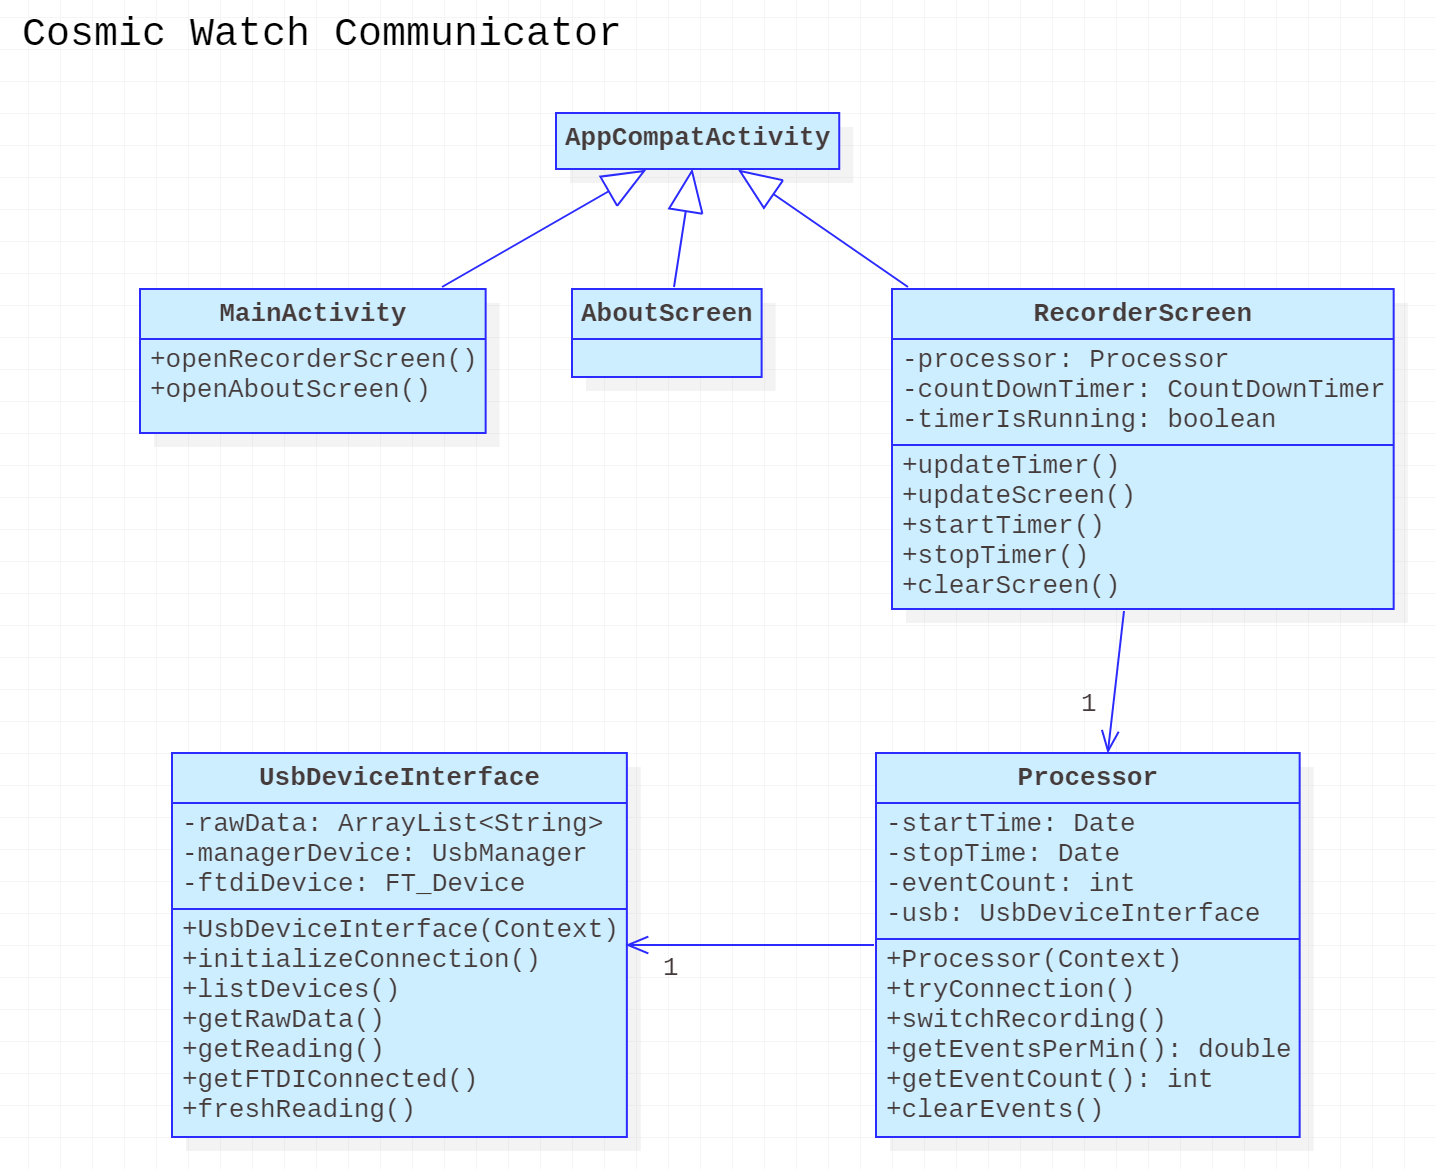
\includegraphics[width=1.5\textwidth]{classes.png}
\end{figure}
\newpage
\subsection*{6-2: Detailed Explanation}

At the top of our diagram, there are three classes extending the class AppCompatActivity. This indicates that these are the main Activities of our app, representing the screens the user can access; MainActivity, AboutScreen and RecorderScreen correspond to the Main Menu, About, and Recorder screens respectively.

The Main Menu screen allows the user to access the About and Recorder screens. Thus, MainActivity has the methods openRecorderScreen and openAboutScreen. The About screen simply displays information, so it does not have relevant attributes and operations to show.

RecorderScreen maintains a reference to a Processor object, which communicates between the UsbDeviceInterface and the RecorderScreen.

The RecorderScreen starts a timer when the user chooses to start recording. This is conveyed to the Processor, which will save the time recording starts and initialize the UsbDeviceInterface. The UsbDeviceInterface will open a wired connection to the muon detector and store raw data from it. When this data needs to be interpreted and displayed on the RecorderScreen, the Processor will make requests to the UsbDeviceInterface and update eventCount according to the amount of raw data saved.

When the recording session timer ends or when the user wishes to clear their saved data, the RecorderScreen sends another signal to Processor. The Processor will then reset its saved data and the raw data in UsbDeviceInterface as needed.


\newpage

\section*{Deliverable \#7}

\subsection*{7-1: Sequence Diagram 1 with Explanation}

\begin{figure}[h] \centering
	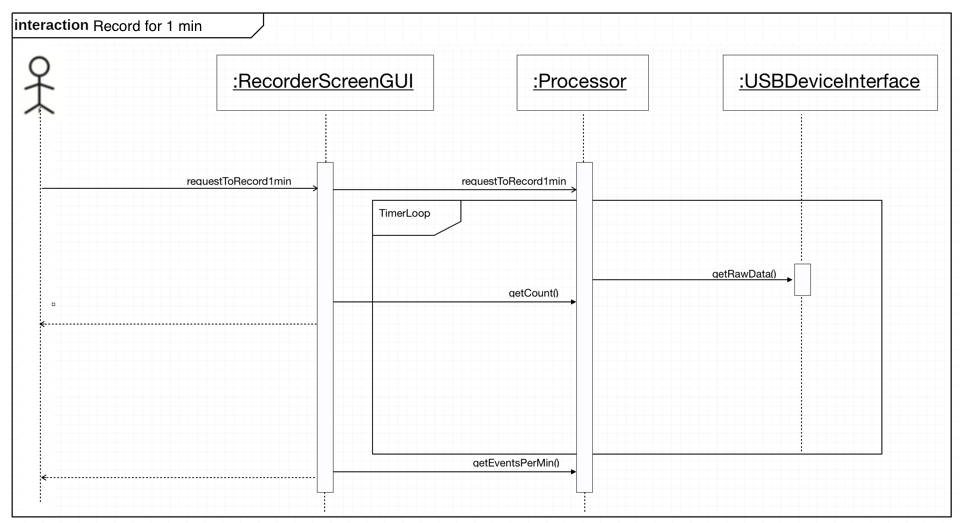
\includegraphics[width=1.08\textwidth]{sequence1.png}
\end{figure}

Our first sequence diagram demonstrates the sequence of tasks where a user initiates a recording for 1 minute. This is done by the user first being able to interact with a RecorderScreenGUI interface, specifically a button. The button communicates with the Processor class which creates a corresponding time stamp for the start of the recording session and enters into a TimerLoop for 60 seconds. During those 60 seconds, the Processor communicates with the USBDeviceInterface, which is a class used to communicate with an external piece of hardware known as a muon detector. 

As the muon detector picks up events, the Processor class calls getRawData() method from the USBDeviceInterface class increment events, which increases the private variable count in the Processor class. This happens every time a muon event occurs during those 60 seconds. The RecorderScreenGUI class then updates the count displayed by calling teh getCount() method from Processor. At the end of the TimerLoop, the RecorderScreenGUI calls the getEventsPerMin() method of the Processor class which calculates the total events that occurred divided by the total duration the recording took place by using the date stamp time difference. 

All of this information is then finally presented to the user in the RecorderScreenGUI. This entire sequence of tasks demonstrates a key concept in software engineering/computer science which is a layer of abstraction with all of the subsystems working behind the scenes while the user only interacts with a friendly UI. 

\newpage
\subsection*{7-2: Sequence Diagram 2 with Explanation}

\begin{figure}[h] \hspace{-2cm}
	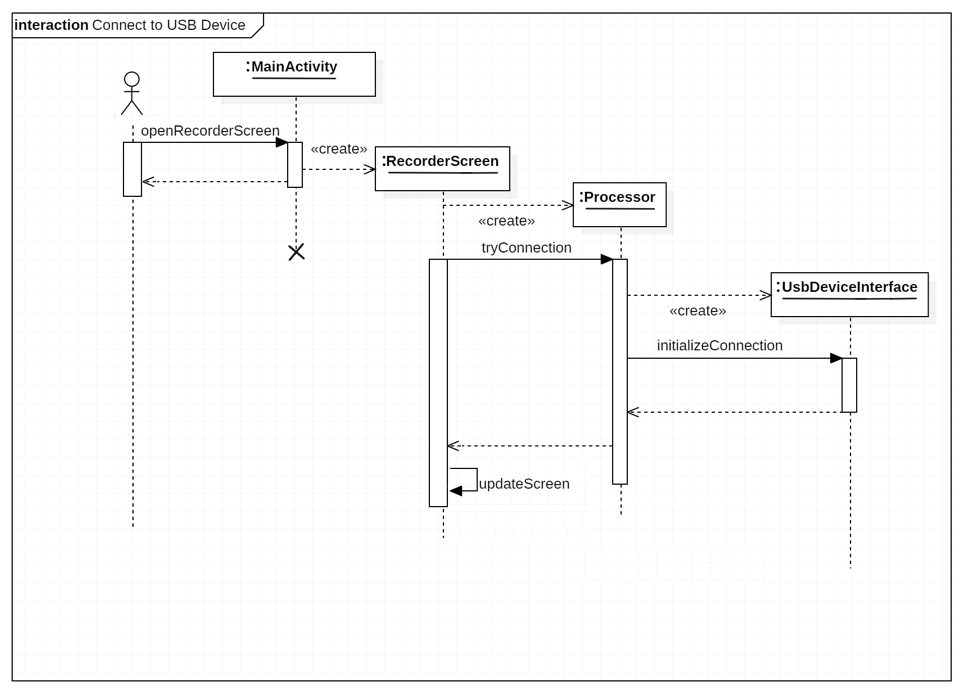
\includegraphics[width=1.3\textwidth]{sequence2.png}
\end{figure}


This sequence diagram shows the use case of the user successfully connecting to the muon detector through a USB port. When the user is on the Main Menu screen (MainActivity), they will choose to open the Recorder screen. This results in an instance of RecorderScreen being created, which also creates a Processor. MainActivity is no longer needed. 

Upon creation, RecorderScreen will ask the Processor to try to connect to the detector using the UsbDeviceInterface. The Processor will initialize the UsbDeviceInterface, and the UsbDeviceInterface will form the connection with the muon detector. After this connection is formed successfully, initializeConnection and tryConnection will return to the RecorderScreen. Finally, the RecorderScreen will display a message using updateScreen to show that the device is connected.



\newpage
\section*{Deliverable \#8}

\subsection*{8-1: Class Diagram with Design Pattern}



\subsection*{8-2: Explanation}





\section*{Deliverable \#9}

See PowerPoint presentation in the submitted .zip file.


\section*{Deliverable \#10}

Collaboration with client blurb.



\end{document}